\chapter{Prototype Application}
\label{prototype}
In order to demonstrate practical use of the models trained in Chapter 4, a prototype application was developed.
This application was developed for a smartphone running on the Android operating system in the Java programming language.
A backend service was created to receive an image from the smartphone application, process the image using the CNN previously developed and return a response to the appliaction in the form of a prediction. ƒff

\section{Requirements}
Lightweight requirements elicitation was carried out for this FYP.
Since prototyping itself is an elicitation technique \parencite{reqs}, the requirements for this prototype application did not need to be extensive.
Myself and my supervisor acted as stakeholders for this project as users of the system.
Two methods of elicitation were used for this project sourced from \parencite{reqs}.
These elicitation techniques were data gathering from an existing system and brain storming.

In a previous FYP, a mobile application was developed for nutritional assessment.
The use of this application provided the opportunity to elicit requirements based on data gathered from this system. Brainstorming also took place between the stakeholders for requirements elicitation.

\tocless\subsection{Functional Requirements}
The functional requirements for this application can be seen in Table \ref{requirements}.

\begin{longtable}{|p{.75cm}|p{3.5cm}|p{6cm}|p{2.5cm}|}
\hline
\textbf{ID} & \textbf{Title}                                              & \textbf{Description}                                                                                    & Dependencies                                   \\ \hline
R1          & Open application from Android phone                         & A user can open the application from a list of applications on their Android phone.                     &                                                \\ \hline
R2          & Choose to take a photo                                      & A user can choose to take a photo of a food item.                                                       & R1                                             \\ \hline
R3          & Take a photo                                                & A user can take a photo using the application.                                                          & R1, R2                                         \\ \hline
R4          & Confirm the photo                                           & A user can confirm the photo captured is sufficient.                                                    & R1, R2, R3                                     \\ \hline
R5          & Retry photo capture                                         & A user can retry the capturing of an image.                                                             & R1, R2, R3                                     \\ \hline
R6          & Send the image to be classified                             & A user can send an image of a food item to be classified.                                               & R1, R2, R3, R4                                 \\ \hline
R7          & Cancel sending an image                                     & A user can cancel sending an image.                                                                    & R1, R2, R3, R4                                 \\ \hline
R8          & Classify the food image                                     & The system can classify an image as a food type.                                                        & R1, R2, R3, R4, R6                             \\ \hline
R9          & View the food image classification                          & A user can view the classification made of the image.                                                   & R1, R2, R3, R4, R6, R8                         \\ \hline
R10         & View the calorie information of the food classification     & A user can view the calorie information of the classified food type.                                    & R1, R2, R3, R4, R6, R8                         \\ \hline
R11         & Change the food classification data                         & A user can change the food classification data if they are unhappy with it.                             & R1, R2, R3, R4, R6, R8, R9                     \\ \hline
R12         & Change the calorie information                              & A user can change the calorie information if they are unhappy with it.                                  & R1, R2, R3, R4, R6, R8, 10                     \\ \hline
R13         & Submit the food classification and calorie data for logging & A user can submit the data calculated such as classification data and calorie information to be logged. & R1, R2, R3, R4, R6, R8, R9, R10                \\ \hline
R14         & Save food log data                                          & The system can save information for logging.                                                            & R1, R2, R3, R4, R6, R8, R9, R10, R13           \\ \hline
R15         & Choose to classify an image from the phone's storage        & A user can choose to select an image from the phone's storage to be classified.                         & R1                                             \\ \hline
R16         & Choose an image from phone's storage                        & A user can choose an image from the phone's storage to classify.                                        & R1, R14                                        \\ \hline
R17         & Choose to view food logs                                    & A user can choose to view the food logs saved on their device.                                          & R1                                             \\ \hline
R18         & View food logs by day                                       & A user can view the food logs saved on the device by day.                                               & R1, R2, R3, R4, R6, R8, R9, R10, R13, R17      \\ \hline
R19         & View food logs by week                                      & A user can view the food logs saved on the device by week.                                              & R1, R2, R3, R4, R6, R8, R9, R10, R13, R17      \\ \hline
R20         & View food logs by month                                     & A user can view the food logs saved on the device by month.                                             & R1, R2, R3, R4, R6, R8, R9, R10, R13, R17      \\ \hline
R21         & View total calories recorded per day                        & A user can view the total calorie count recorded per day.                                               & R1, R2, R3, R4, R6, R8, R9, R10, R13, R17      \\ \hline
R22         & View total calories recorded per week                       & A user can view the total calorie count recorded per week.                                              & R1, R2, R3, R4, R6, R8, R9, R10, R13, R17      \\ \hline
R23         & View total calories recorded per month                      & A user can view the total calorie count recorded per month.                                             & R1, R2, R3, R4, R6, R8, R9, R10, R13, R17      \\ \hline
R24         & Delete a food log                                           & A user can delete an individual food log.                                                               & R1, R2, R3, R4, R6, R8, R9, R10, R13, R17, R18 \\ \hline
\caption{Functional Requirements}
\label{requirements}
\end{longtable}

\tocless\subsection{Non-Functional Requirements}
The nature of a prototype application does not call for non-functional requirements.
Despite this, some non-functional requirements were kept in mind during the development of this application such as:
\begin{itemize}
	\item{Performance - for example, how long it takes for an image to be classified.}
	\item{Extensibility - is it easy to extend the functionality of the system.}
	\item{Maintainability - how easy it is to maintain the system.}
	\item{Usability - how easy it is to use the system.}
\end{itemize}

\clearpage

\section{Design}
The design process for this prototype application consisted of user interface design, android application system design and the activity of choosing resources for a backend host.

\subsection*{User Interface}
The user interface mock ups were created using \parencite{fluid}.
The aim of this design was to provide a simple, easy to use interface so that a user could use the application with minimal effort.
The main benefit of using computer vision for this type of application is to
reduce the effort of the user or dietician keeping track of food intake.
Therefore, this application had to be very quick and easy to use.
The application is called NutriLog.

Three main activities were needed for this application.
The first activity, as seen in Figure \ref{fig:page1}, would consist of options to either take an image of food or to view the food logs of the user.
If the user decides to take an image of food, they will be brought to the second activity which can be seen in Figure \ref{fig:page2}.
The user is required to take a picture before reaching the activity in Figure \ref{fig:page2}.
Once the user presses the send button the image is classified and the content of the activity changes to display the classification and calorie count as in Figure \ref{fig:page3}.
Alternatively, the user can cancel the process and return to the first activity.
The user would then submit the food classification for logging and automatically return to the first activity.
The final activity is displayed when a user views their food logs.
This activity has the ability to view a list of the food logs taken by the user by day, week or month.
The calorie count of the selected time frame is to be displayed on this activity also.

\begin{figure}[h] 
  \label{ fig7} 
  \begin{minipage}[b]{0.5\linewidth}
    \centering
    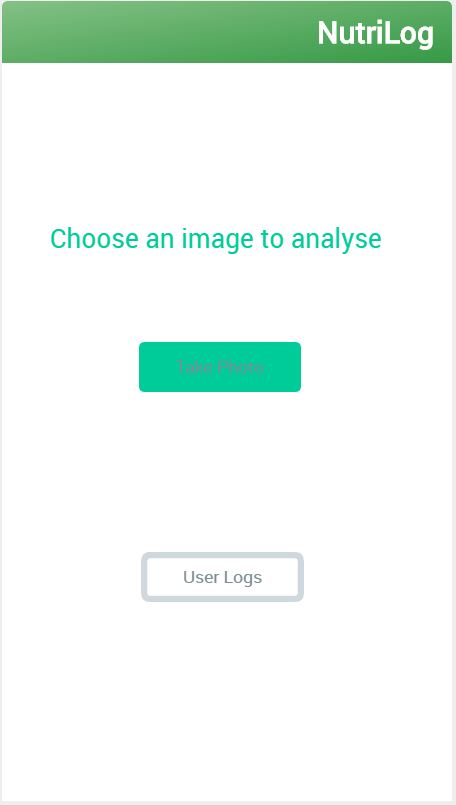
\includegraphics[width=.75\linewidth]{Mockup1} 
    \caption{Landing Activity} 
  \label{fig:page1}
    \vspace{4ex}
  \end{minipage}%%
  \begin{minipage}[b]{0.5\linewidth}
    \centering
    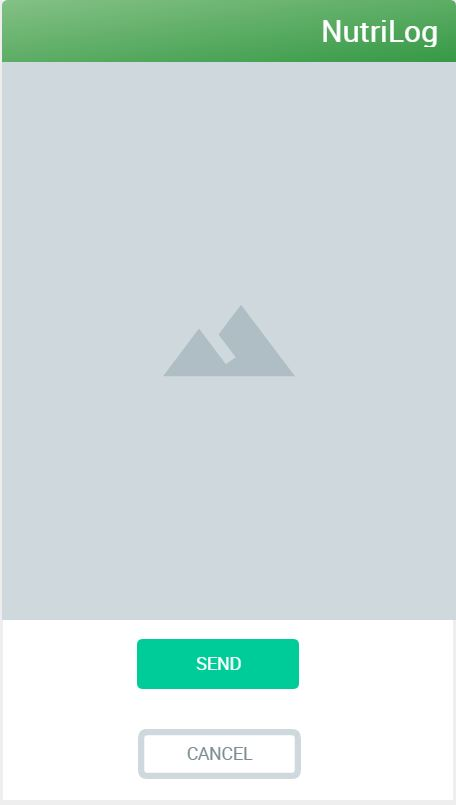
\includegraphics[width=.75\linewidth]{Mockup2} 
    \caption{Image Submission Activity} 
  \label{fig:page2}
    \vspace{4ex}
  \end{minipage} 
  \begin{minipage}[b]{0.5\linewidth}
    \centering
    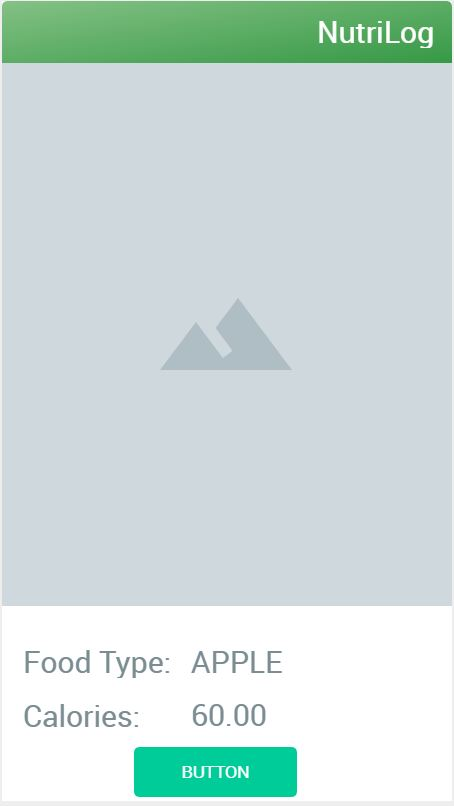
\includegraphics[width=.75\linewidth]{Mockup3} 
    \caption{Classification Activity} 
    \label{fig:page3}
    \vspace{4ex}
  \end{minipage}%% 
  \begin{minipage}[b]{0.5\linewidth}
    \centering
    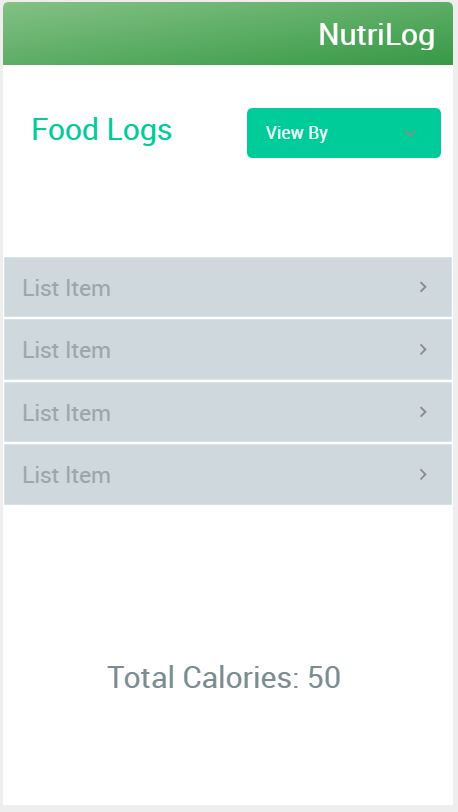
\includegraphics[width=.75\linewidth]{Mockup4} 
    \caption{Food Logs Activity} 
    \label{fig:page4}
    \vspace{4ex}
  \end{minipage} 
\end{figure}
\afterpage{\clearpage}

\subsection*{System Architecture}

\begin{figure}[h]
    \centering
    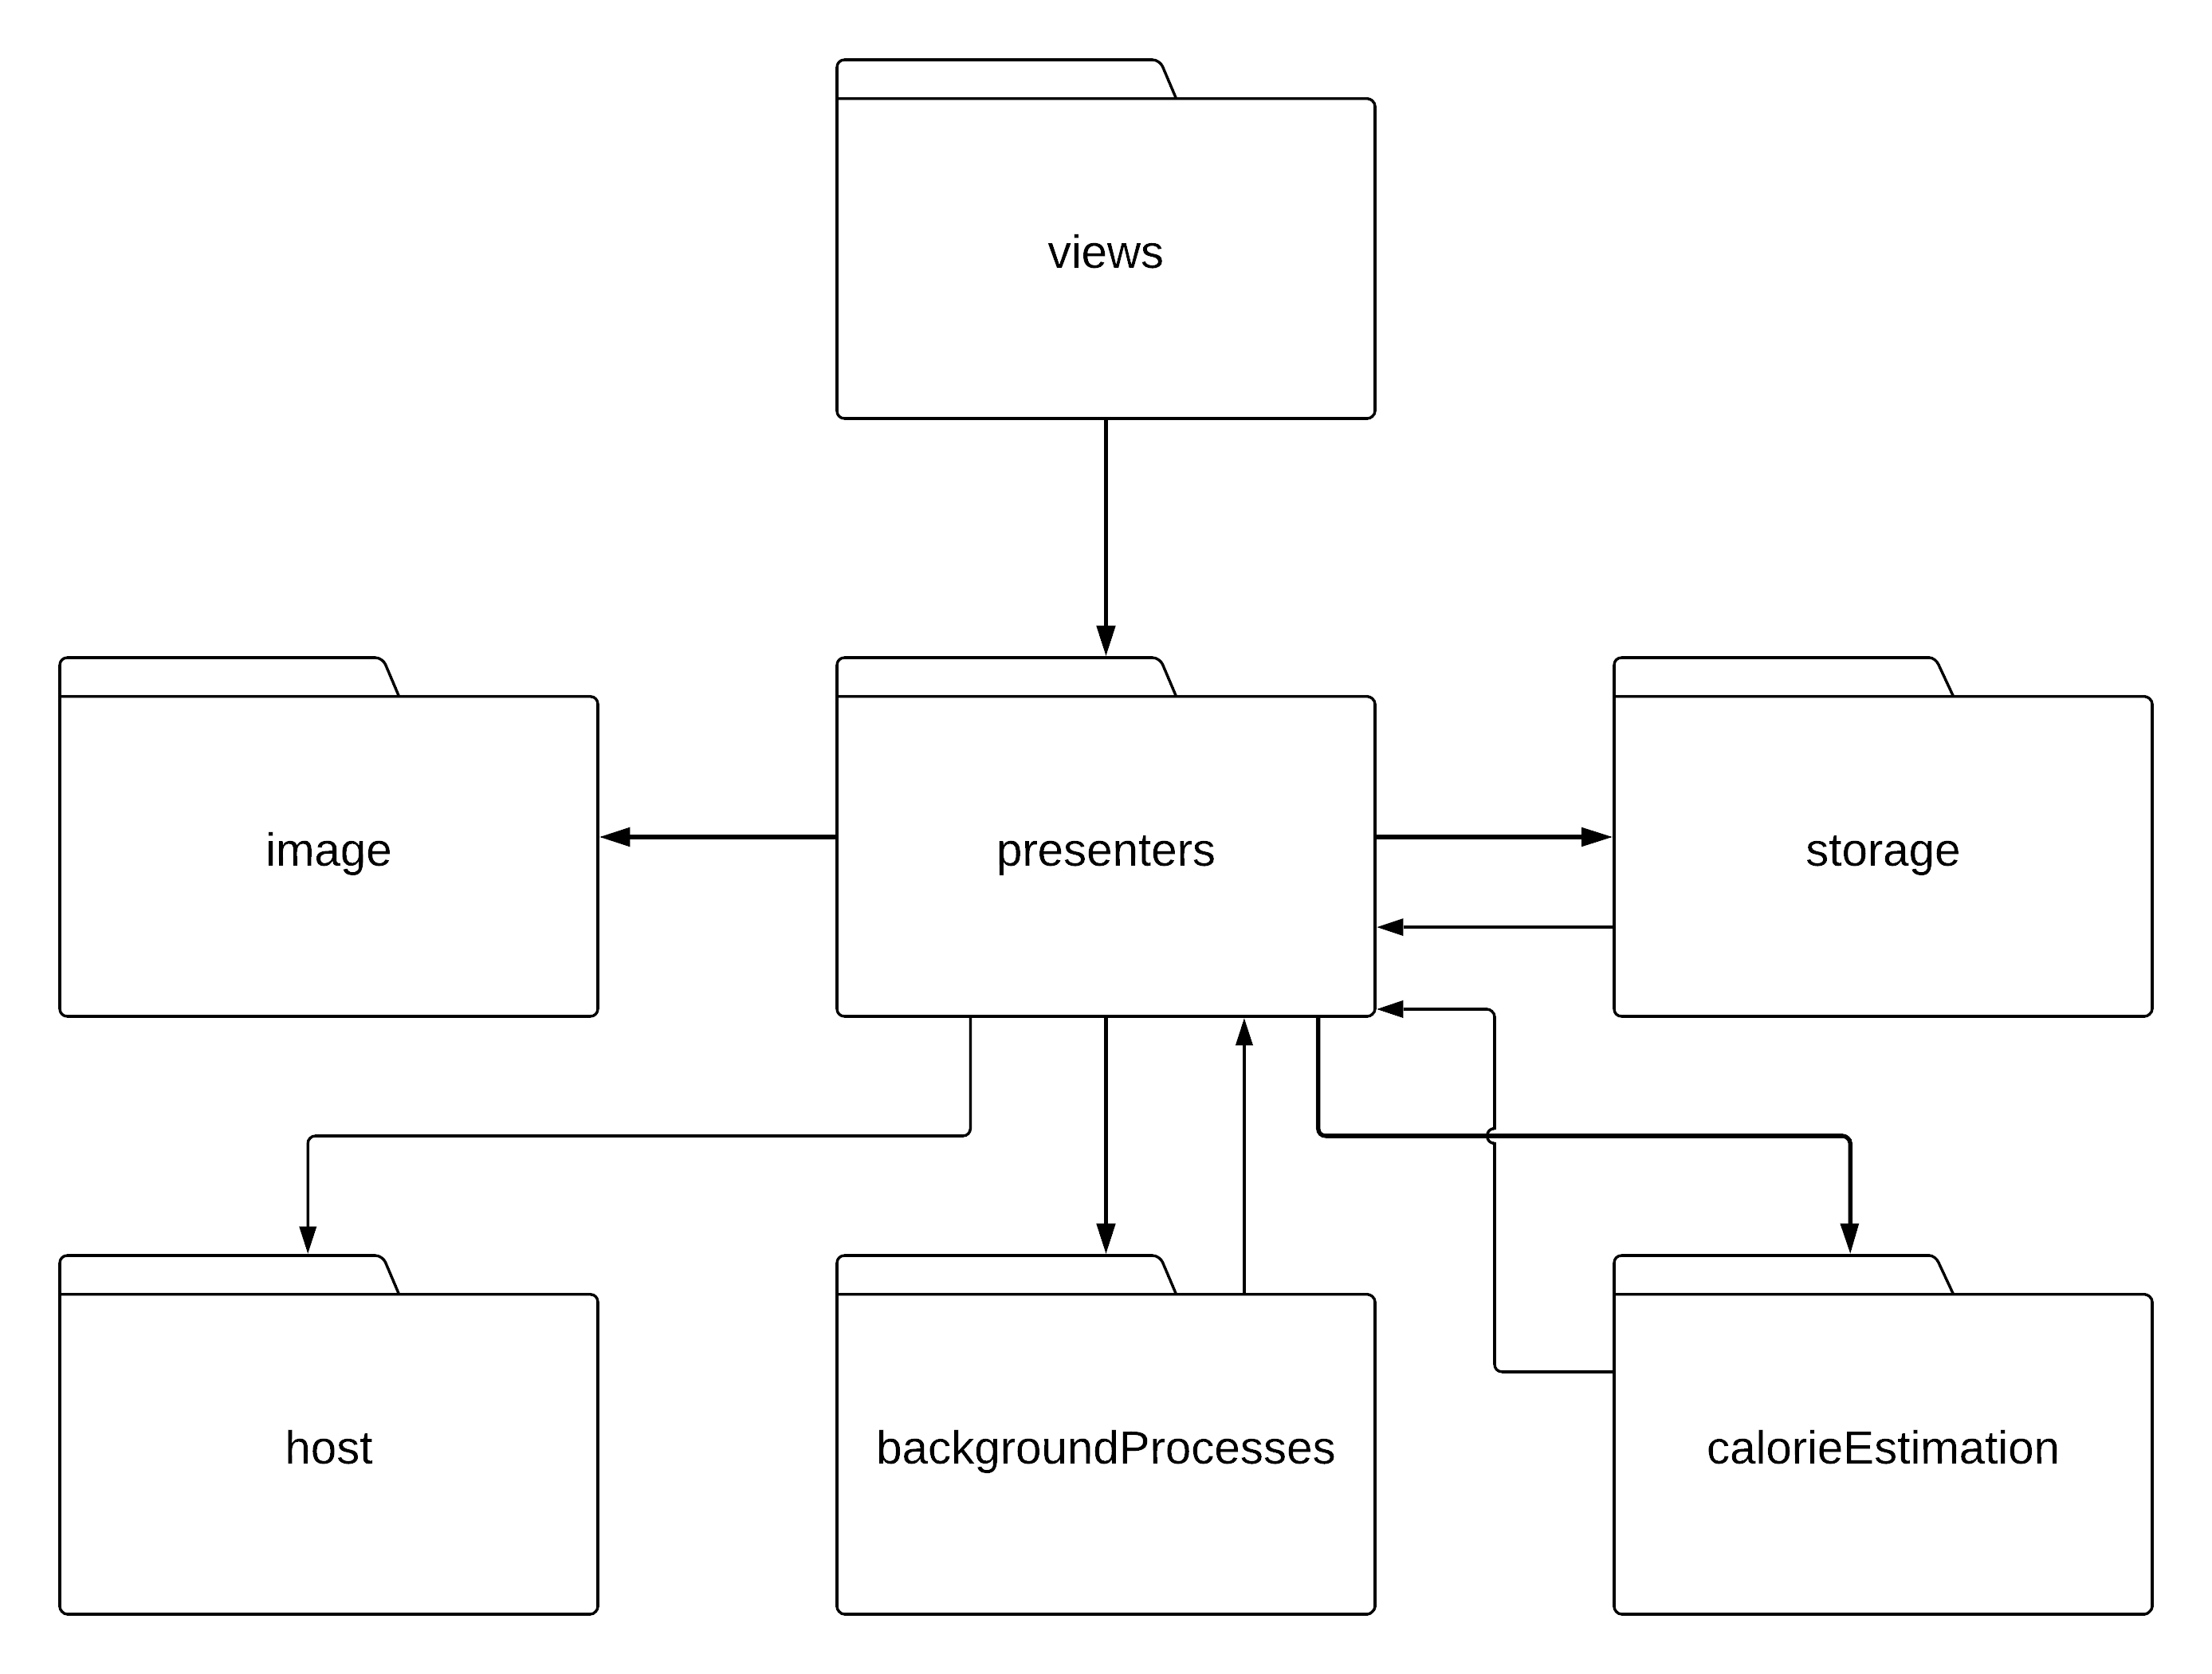
\includegraphics[scale=0.15]{packageDiagram}
    \caption{Package Diagram}
    \label{fig:packageDiagram}
\end{figure}

\subsubsection*{Architectural Patterns}
The Model-View-Presenter (MVP) architectural pattern was adapted for this application \parencite{mvp}.
This pattern is very similar to the Model-View-Controller (MVC) architecture which is quite popular in the software development industry.
The main difference between MVC and MVP is that whereas in MVC the controller is responsible for which view is used, in MPV the presenter is called through the view.
This is due to the architecture of Android applications in general, where the view takes primary control.
In the view classes, there should be no logic whatsoever in an MVP architecture and all logic should be called in the presenters.
There is also a one to one dependency between views and presenters.

As illustrated in Figure \ref{fig:packageDiagram}, the views in the application
have a dependency only on their corresponding presenter.
The presenters contain the business logic of the  application and have a dependency on all other packages.
The packages of backgroundProcesses, calorieEstimation and storage have a dependancy on the presenters package for callback purposes and also database creation in Android requires context of the activity information.

\subsubsection*{Marchitecture}
In Figure \ref{fig:market}, a marchitecture diagram can be seen.
This diagram represents the architecture of the system.
NutriLog is an Android application that send an image to an AWS (Amazon Web Services) instance using the API OkHttp. The AWS instance is running a Python FLASK application that classifies the image using a TensorFlow model and sends a response back to NutriLog. The Nutritionix API is used to collect nutritional information of this classification.

\begin{figure}[h]
    \centering
    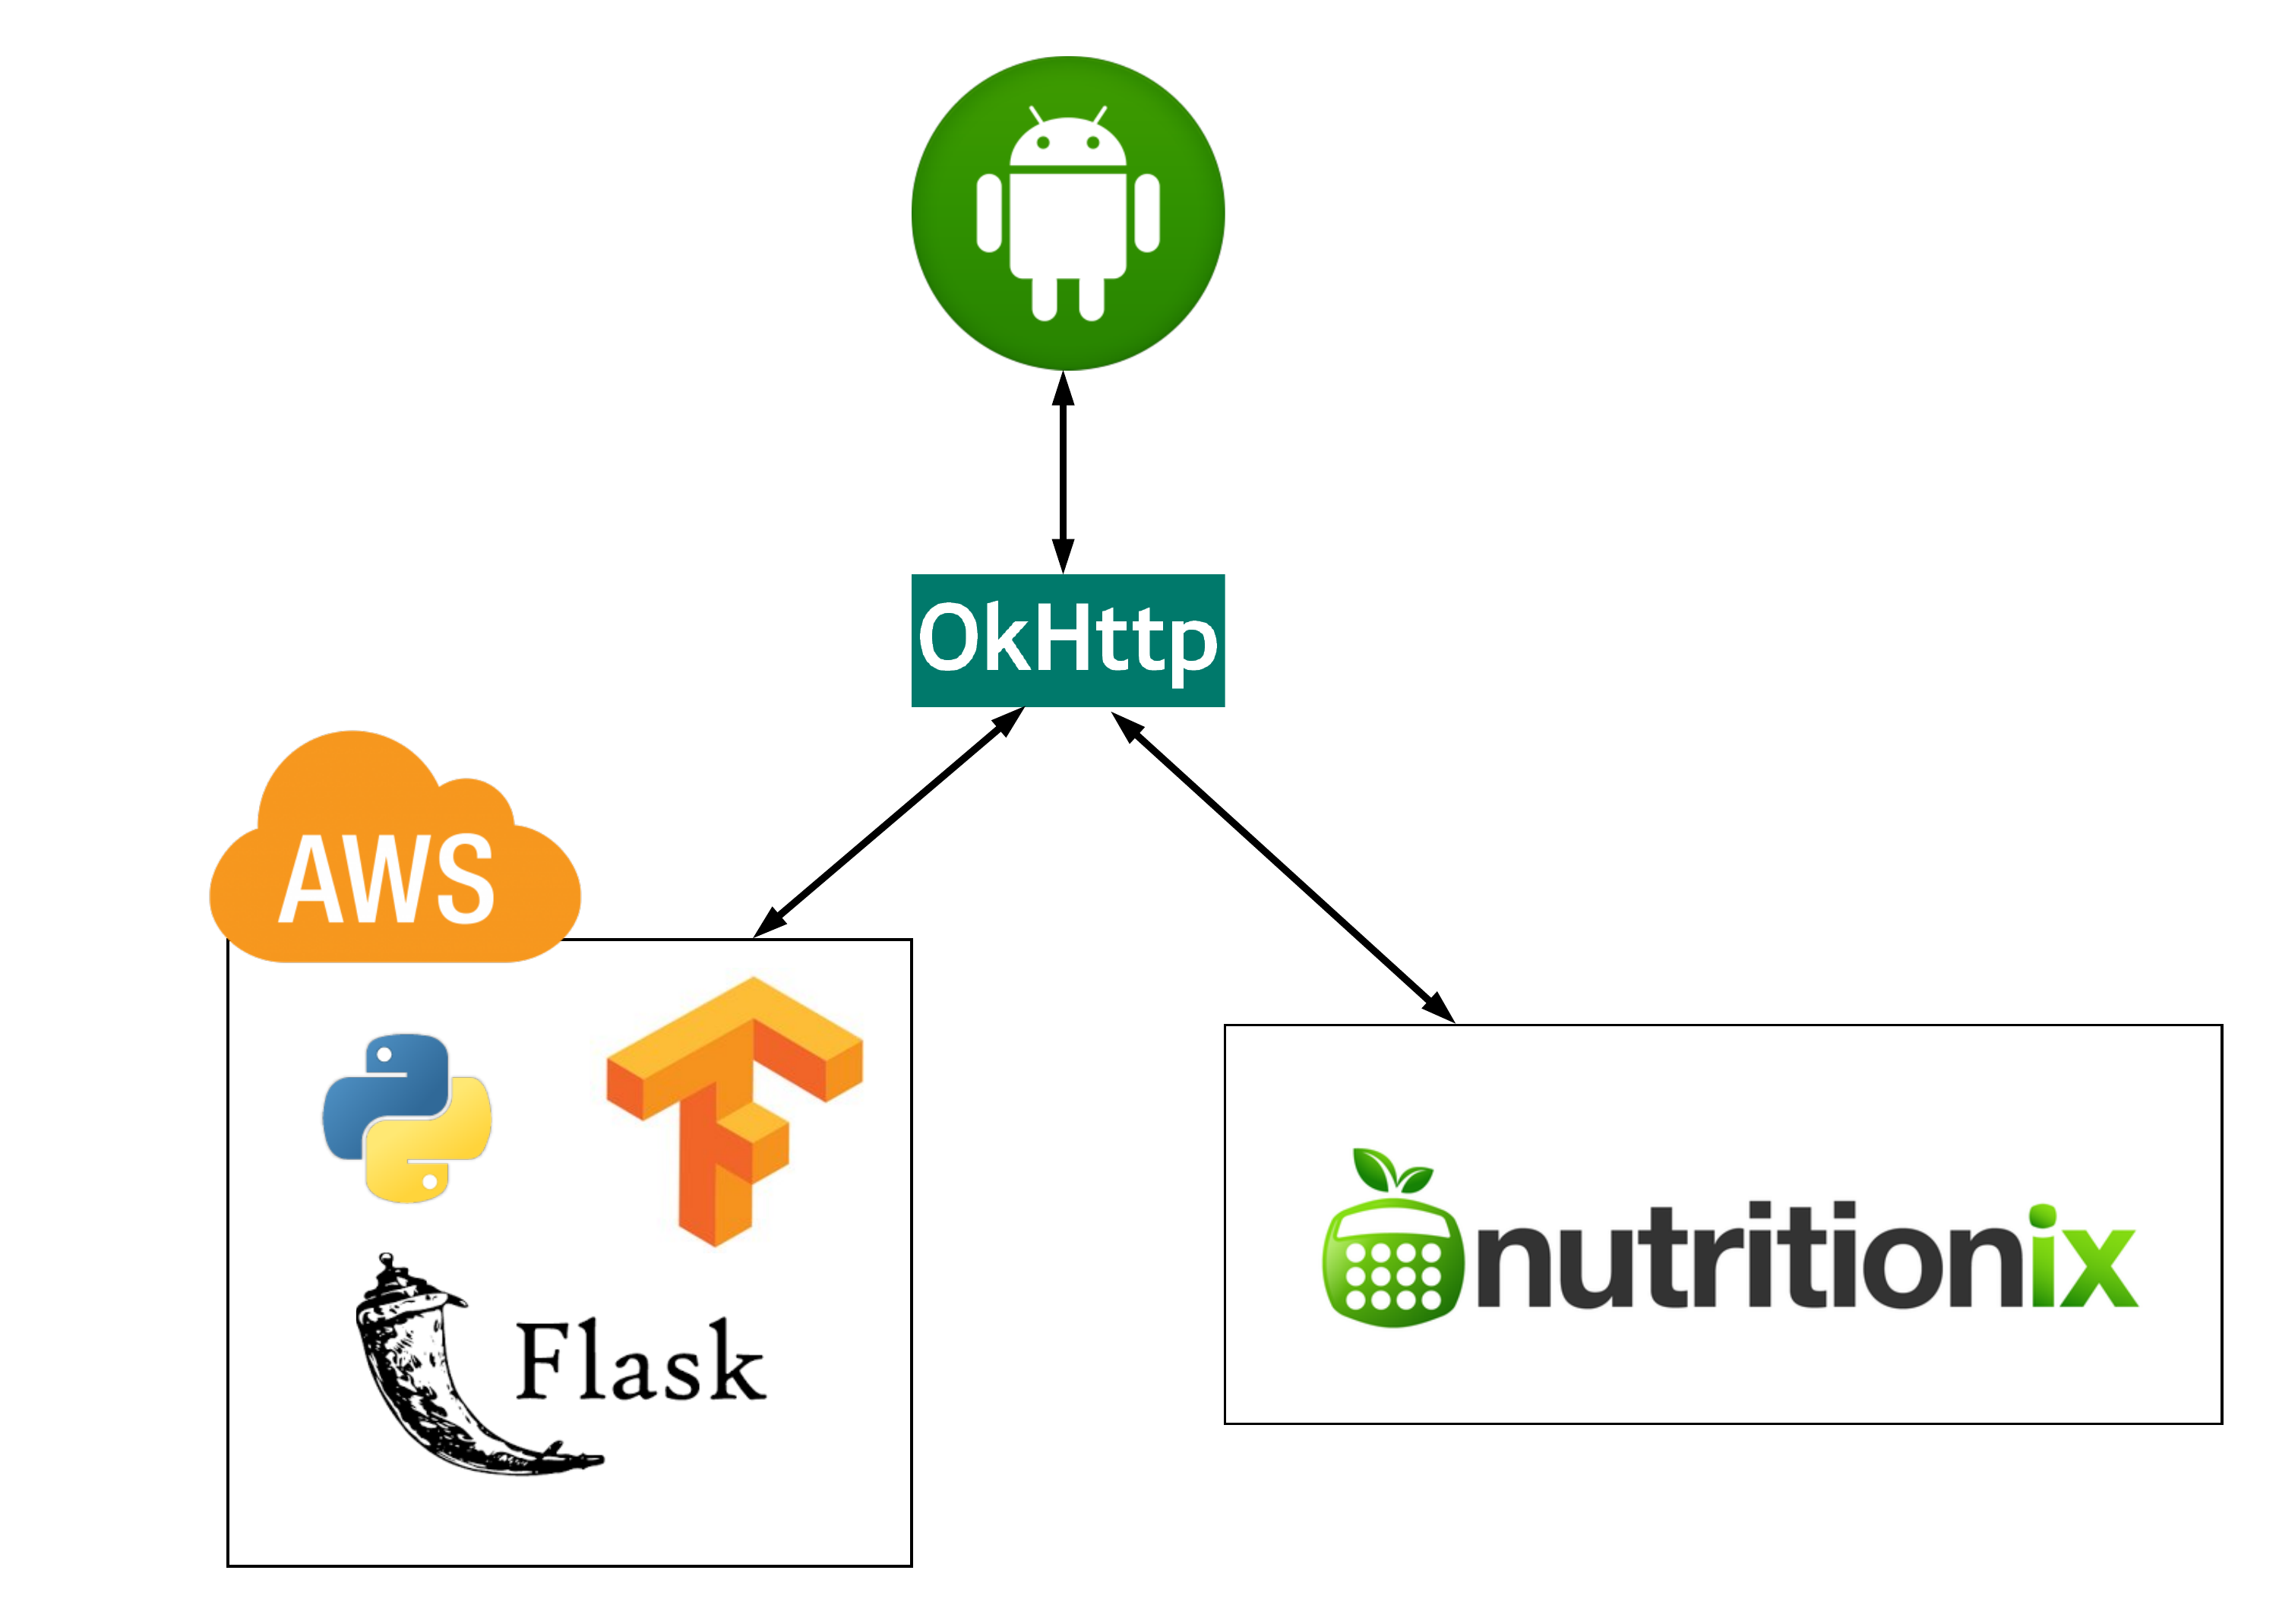
\includegraphics[scale=0.15]{market}
    \caption{Marchitecture Diagram}
    \label{fig:market}
\end{figure}

The technologies used for this appliction were used for the following reasons:

\textbf{AWS}
\linebreak
Past experience was a large factor when it came to choosing a cloud provider to host the backend instance for this prototype application.
AWS instances are very easy to set up once the process has been carried out a few times and this was a contributing factror to why AWS was chosen.
AWS also has a free tier which provides all the necessary server space to host the backend service for this application.

\textbf{OkHttp}
\linebreak
OkHttp seemed to be popular for Android applications as seen on websites such as Stack Overflow.
OkHttp also has extensive documentation and is a very simple API to import into Android.
The learning curve for OkHttp is quite small and it doesn't require much code to carry out a simple task like sending a HTTP POST request to a backend instance.

\textbf{FLASK}
\linebreak
Python FLASK was used for the backend service in this FYP due to past experience and its simplicity.

\textbf{TensorFlow}
\linebreak
TensorFlow was chosen as the library to create neural networks for this FYP mostly because of its reputation.
TensorFlow has been used by many researches in the computer vision industry.
TensirFlow also has extensive documentation and a wide array or resources and tutorials.

\textbf{Nutritionix}
\linebreak
Nutrionix was the best nutrional information API that was also free to use and this is why it was chosen.

\section{Implementation}
Outlined below are some coding fragments categorised under: Design Patterns, Asynchronous Tasks, Presenters, Views and Interesting Coding Fragments.

\tocless\subsection{Design Patterns}
Various design patterns were used in the implementation of this application such as the Factory, the Builder and the Singleton which are outlined below.

The Factory design pattern was used to retrieve a DAO (Data Access Object) as seen in Figure \ref{lst:daoFactory}.
This was used so that if at a future time the storage type of the application is to be changed, the developer would only have to change one instance of the codebase and return a new implementation of the DAO interface in the method getDAO().
\begin{figure}[h]
\caption{DAO Factory Class}
\label{lst:daoFactory}
\begin{lstlisting}[style=Java]
public class DAOFactory {

    public DAO getDAO(Context context){
        return SqlLiteDAO.getInstance(context);
    }
}
\end{lstlisting}
\end{figure}

A Host builder was used to create a Host object.
This builder is a static inner class in the Host class file as documented in Figure \ref{lst:hostBuilder}
\begin{figure}[h]
\caption{HostBuilder Class}
\label{lst:hostBuilder}
\begin{lstlisting}[style=Java]
public static class HostBuilder {
    private final String ipv4;
    private String dns;
    private int port;
    private String route;

    public HostBuilder(String ipv4) {
        this.ipv4 = ipv4;
    }

    public HostBuilder withDns(String dns) {
        this.dns = dns;
        return this;
    }

    public HostBuilder withPort(int port) {
        this.port = port;
        return this;
    }

    public HostBuilder withRoute(String route) {
        this.route = route;
        return this;
    }

    public Host build() {
        return new Host(this);
    }

}
\end{lstlisting}
\end{figure}

A Singleton instance of the DAO implementation was used in this application.
This was mainly due to the best practice of keeping database access objects as singleton instances.
This class can be seen in Figure \ref{lst:singletonDao}.

\begin{figure}[h]
\caption{Singleton DAO Object}
\label{lst:singletonDao}
\begin{lstlisting}[style=Java]
public static DAO getInstance(Context context) {
    if(instance == null) {
        instance = new SqlLiteDAO(context);
    }
    return instance;
}
\end{lstlisting}
\end{figure}

\tocless\subsection{Asynchronous Tasks}
Asynchronous Tasks in Android are used to run tasks in the background or are sometimes used to simply distribute processes off the main thread.
The AsyncTask class must be extended on creation of the background processes.
An AsyncTask was used to send the food image to the backend host as in Figure \ref{lst:rrCode}.
\begin{figure}[h]
\caption{UploadImage Class}
\label{lst:rrCode}
\begin{lstlisting}[style=Java]
@Override
protected String doInBackground(Void... params) {
    String result = "";
    OkHttpClient client = new OkHttpClient();
    String imageToSend = image;
    RequestBody requestBody = new MultipartBody.Builder()
            .setType(MultipartBody.FORM)
            .addFormDataPart("image", imageToSend)
            .build();

    Request request = new Request.Builder().url(host.getUrl())
            .post(requestBody).build();

    Response response = null;
    try {
        response = client.newCall(request).execute();
        result = response.body().string();
        response.body().close();
    } catch (IOException e) {
        e.printStackTrace();
    }

    return result;
}
\end{lstlisting}
\end{figure}

\tocless\subsection{Presenters}
In the MPV architecture as described earlier, the presenter for each activity contains all the logic for that view.
The presenter in Figure \ref{lst:pres} was tasked with creating intents to new activities (views).
\begin{figure}[h]
\caption{MainPresenter Class}
\label{lst:pres}
\begin{lstlisting}[style=Java]
public class MainPresenter {

    private Intent intent;
    private Context context;

    public MainPresenter(Context context) {
        this.context=context;
    }

    public void takePhoto() {
        intent = new Intent(context, CaptureImageActivity.class);
        context.startActivity(intent);
    }

    public void userLogs() {
        intent = new Intent(context, FoodLogsActivity.class);
        context.startActivity(intent);
    }

}
\end{lstlisting}
\end{figure}

\tocless\subsection{Views}
In the MPV architecture that this application uses, the views are responsible for interacting directly with the user interface.
The view for the MainActivity in Figure \ref{lst:mainView} responds to button clicks and calls to its presenter to carry out the logic of the required task.
\begin{figure}[h]
\caption{MainActivity Class}
\label{lst:mainView}
\begin{lstlisting}[style=Java]
public class MainActivity extends AppCompatActivity {

    private MainPresenter mainPresenter;

    @Override
    protected void onCreate(Bundle savedInstanceState) {
        super.onCreate(savedInstanceState);
        setContentView(R.layout.activity_main);

        mainPresenter = new MainPresenter(this);
    }

    public void onClickTakePhoto(View view) {
        mainPresenter.takePhoto();
    }

    public void onClickUserLogs(View view) {
        mainPresenter.userLogs();
    }
}
\end{lstlisting}
\end{figure}

\tocless\subsection{Storage}
SQLite was used for storing data in this application and the class that handled creation, input and output to this database implemented the DAO interface.
An interface for storage devices was created so that each implementation would have the ability to add food logs, retrieve food logs, delete food logs and remove the data store completely.
This is documented in Figure \ref{lst:daoInterface}.
\begin{figure}[h]
\caption{DAO Interface}
\label{lst:daoInterface}
\begin{lstlisting}[style=Java]
public interface DAO {
    void addFoodLog(FoodLog foodLog);
    List<FoodLog> getLogsByDay(Date date);
    List<FoodLog> getLogsByWeek(Date date);
    List<FoodLog> getLogsByMonth(Date date);
    void deleteFoodLogs(List<FoodLog> foodLogs);
    void deleteDb();
}
\end{lstlisting}
\end{figure}

The method in Figure \ref{lst:getLogs} was used to execute a query and return a List of FoodLog objects.
\begin{figure}[h]
\caption{Get Food Logs Per Date}
\label{lst:getLogs}
\begin{lstlisting}[style=Java]
@Override
private List<FoodLog> selectQuery(String query) {
        foodLogs = new ArrayList<>();
        Cursor resultSet = database.rawQuery(query, null);
        while(resultSet.moveToNext()) {
            try {
                foodLogs.add(new FoodLogImpl
                .FoodLogBuilder(resultSet.getString(1))
                .withId(resultSet.getInt(0))
                .withCalories(resultSet.getDouble(2))
                .withTimestamp(dateFormat
                    .parse(resultSet.getString(3)))
                .build());
            } catch (ParseException e) {
                e.printStackTrace();
            }
        }
    return foodLogs;
}
\end{lstlisting}
\end{figure}

\tocless\subsection{Interesting Coding Fragments}
Some interesting coding fragments are outlined below which merit inclusion in this report.

The method in Figure \ref{lst:encodeBitmap} was used to encode the image taken on the phone to a string.
This was used to send the image to the backend with minimal latency.
The bitmap size was also reduced as in line 8 to decrease response time also.
\begin{figure}[h]
\caption{Encode Bitmap to base64 String}
\label{lst:encodeBitmap}
\begin{lstlisting}[style=Java]
public String toBase64() {
    BitmapFactory.Options options = new BitmapFactory.Options();
    options.inSampleSize = 8;

    Bitmap imageBitmap = BitmapFactory.decodeFile(image.getAbsolutePath(), options);

    //resize image for faster upload to server
    Bitmap.createScaledBitmap(imageBitmap, 300, 400, false);
    
    ByteArrayOutputStream byteArrayOutputStream = new ByteArrayOutputStream();
    imageBitmap.compress(Bitmap.CompressFormat.PNG, 100, byteArrayOutputStream);
    byte[] byteArray = byteArrayOutputStream.toByteArray();

    return Base64.encodeToString(byteArray, Base64.DEFAULT);
}
\end{lstlisting}
\end{figure}

A map of strings to runnables was used to query the database for food logs as documented in Figure \ref{lst:map}.
This was used as the select query for the database had to dynamically change depending on how the food logs were being viewed, by day, week, or month.
\begin{figure}[h]
\caption{Map of Runnables}
\label{lst:map}
\begin{lstlisting}[style=Java]
listViewOptions = new HashMap<>();
listViewOptions.put("Day", () -> getLogsByDay());
listViewOptions.put("Week",() -> getLogsByWeek());
listViewOptions.put("Month", () -> getLogsByMonth());
\end{lstlisting}
\end{figure}

\tocless\subsection{User Interface}
User interface implementation as in Figures \ref{fig:gallery}, \ref{fig:ui2}, \ref{fig:ui3}, \ref{fig:ui5}, \ref{fig:ui8}, \ref{fig:ui6}, \ref{fig:ui7} and \ref{fig:delete}.

\begin{figure}
  \label{uiDesign1} 
  \begin{minipage}[b]{0.5\linewidth}
    \centering
    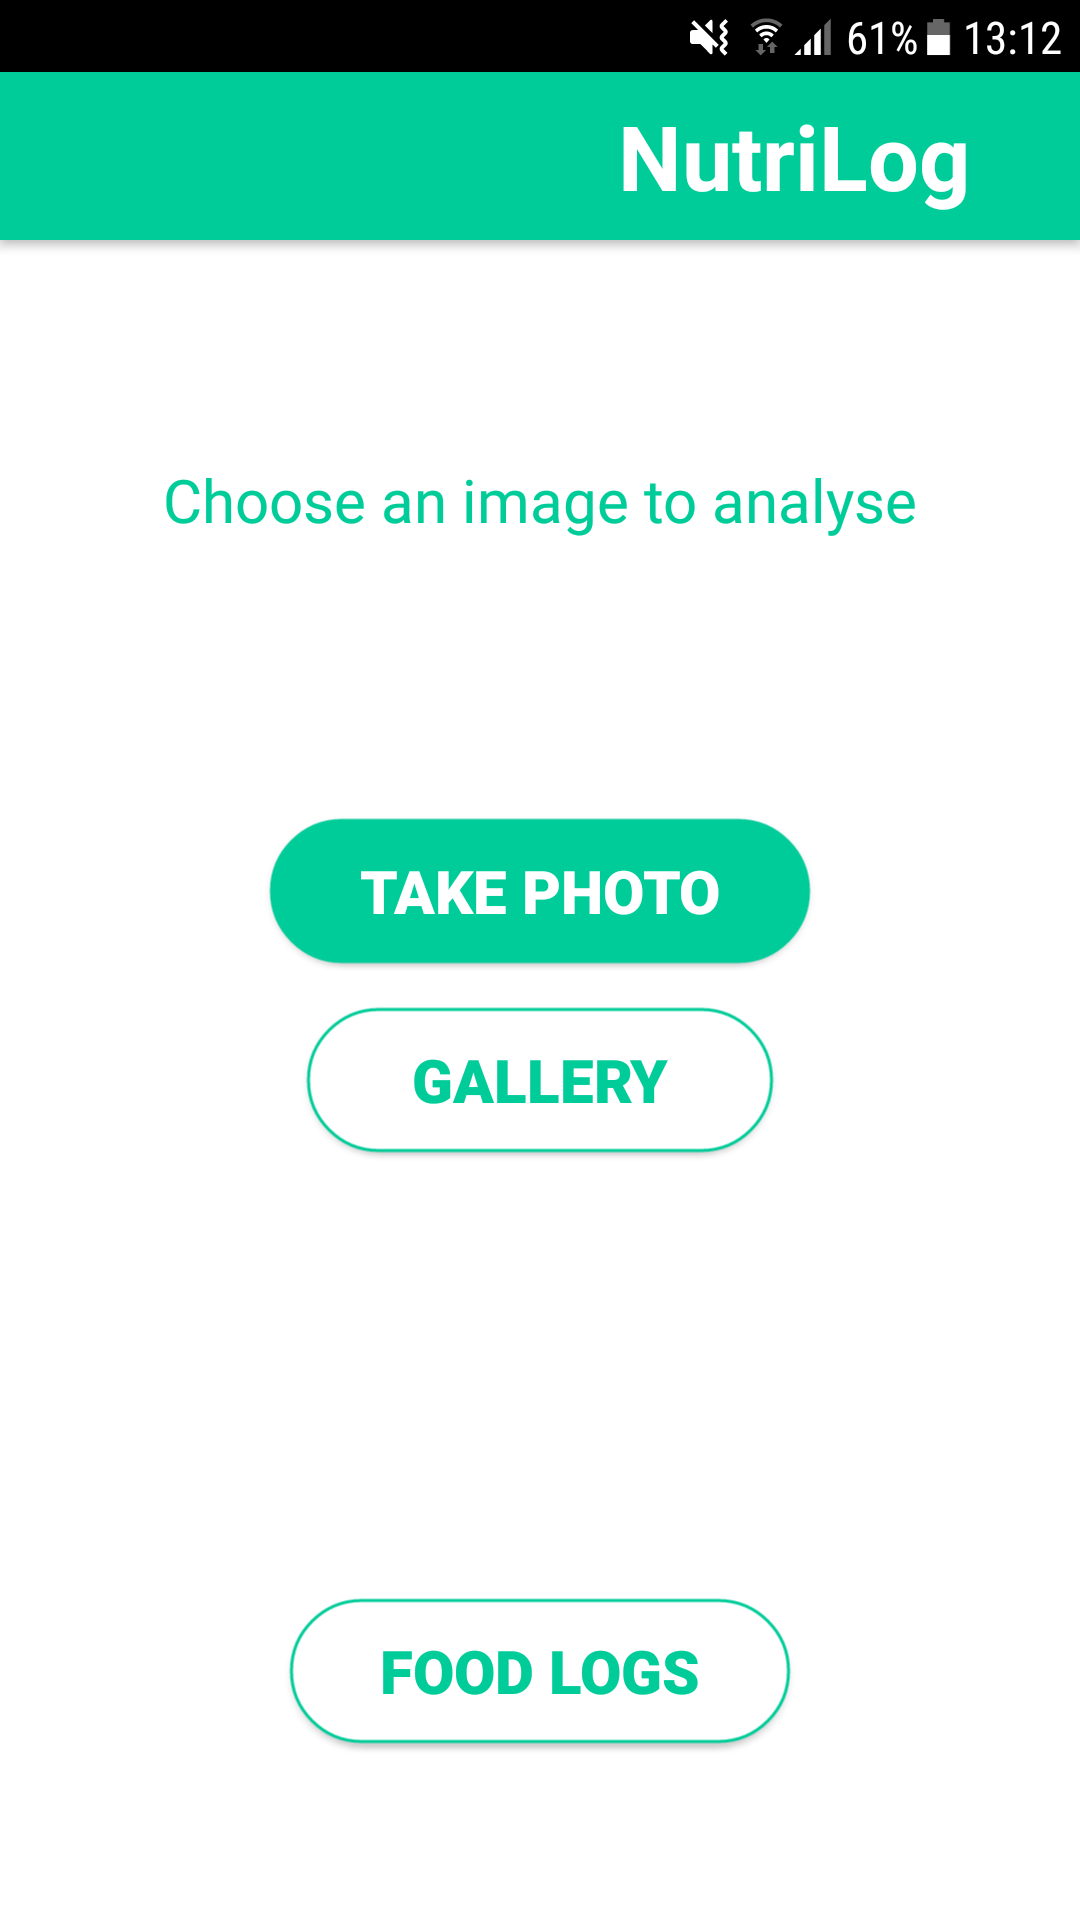
\includegraphics[width=.75\linewidth]{gallery} 
    \caption{Landing Activity} 
  \label{fig:gallery}
    \vspace{4ex}
  \end{minipage}%%
  \begin{minipage}[b]{0.5\linewidth}
    \centering
    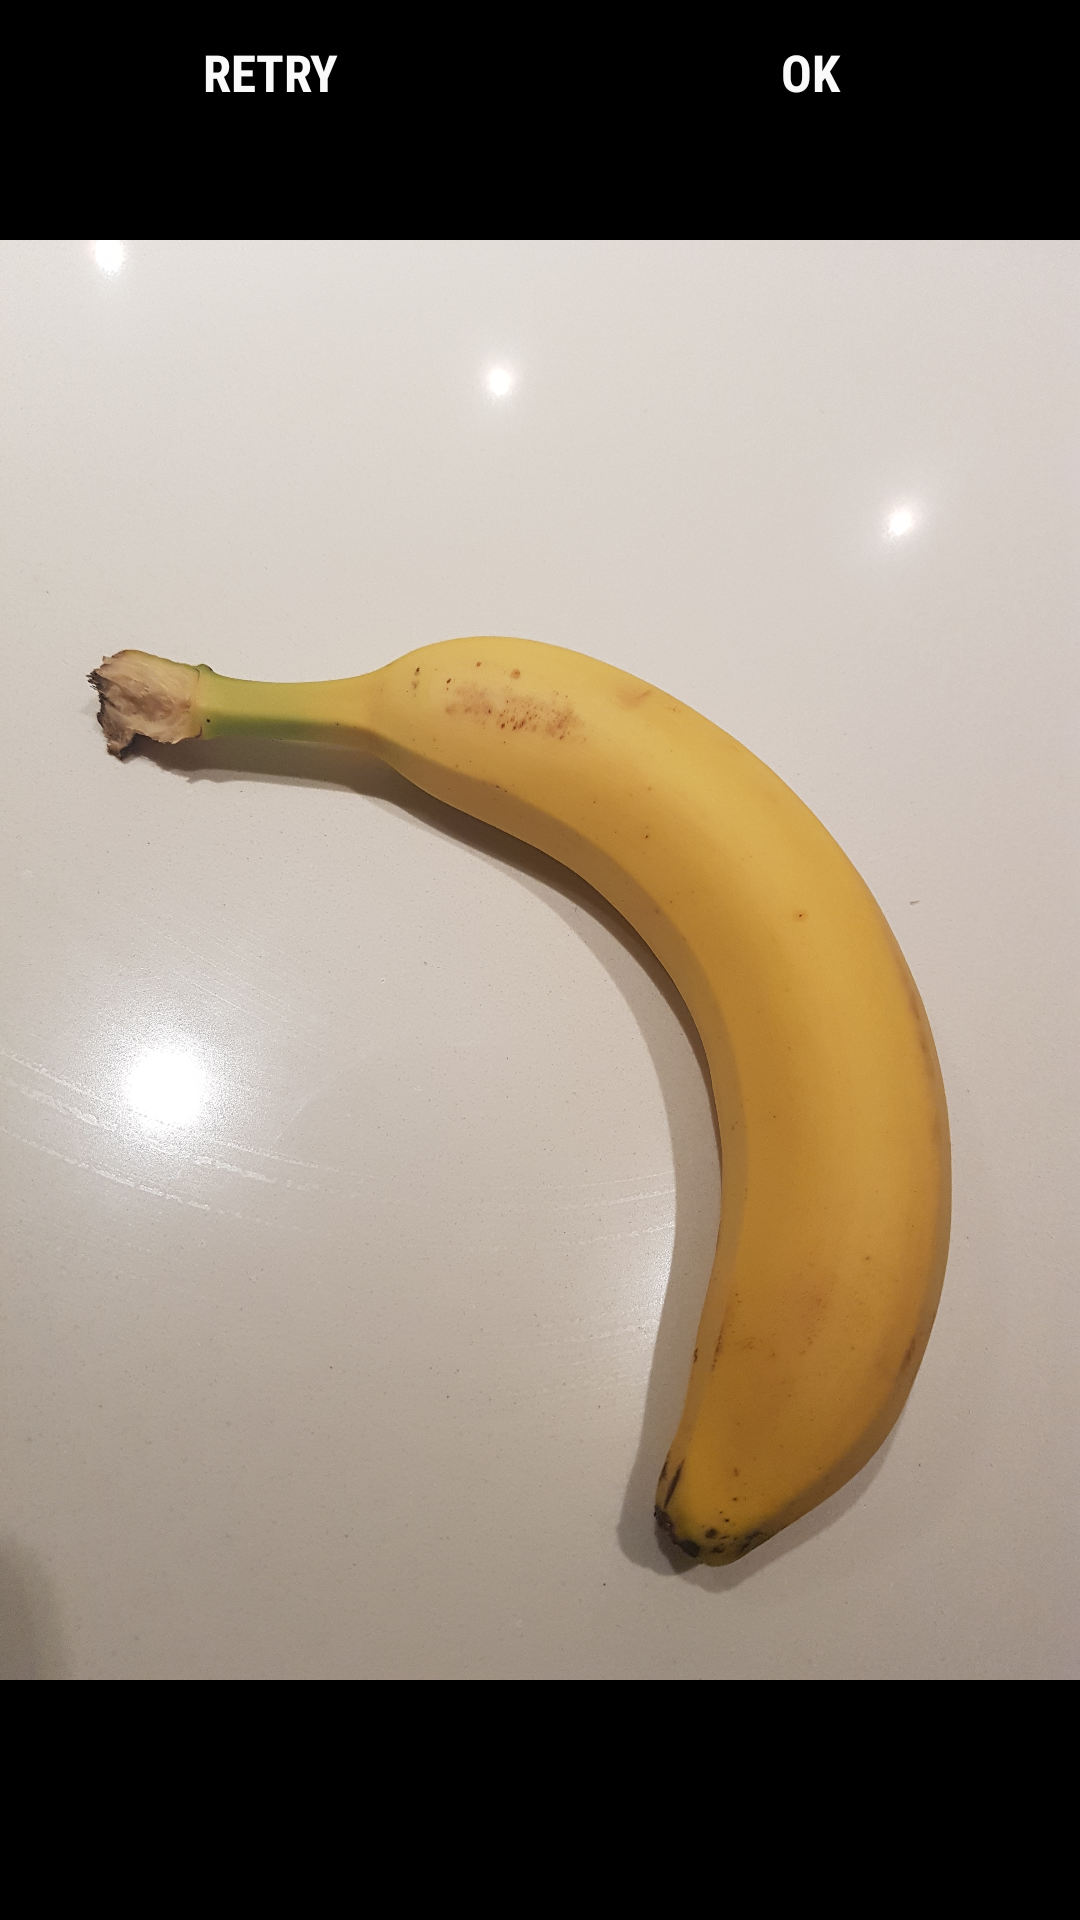
\includegraphics[width=.75\linewidth]{ui2} 
    \caption{Image Capture Activity} 
  \label{fig:ui2}
    \vspace{4ex}
  \end{minipage} 
  \begin{minipage}[b]{0.5\linewidth}
    \centering
    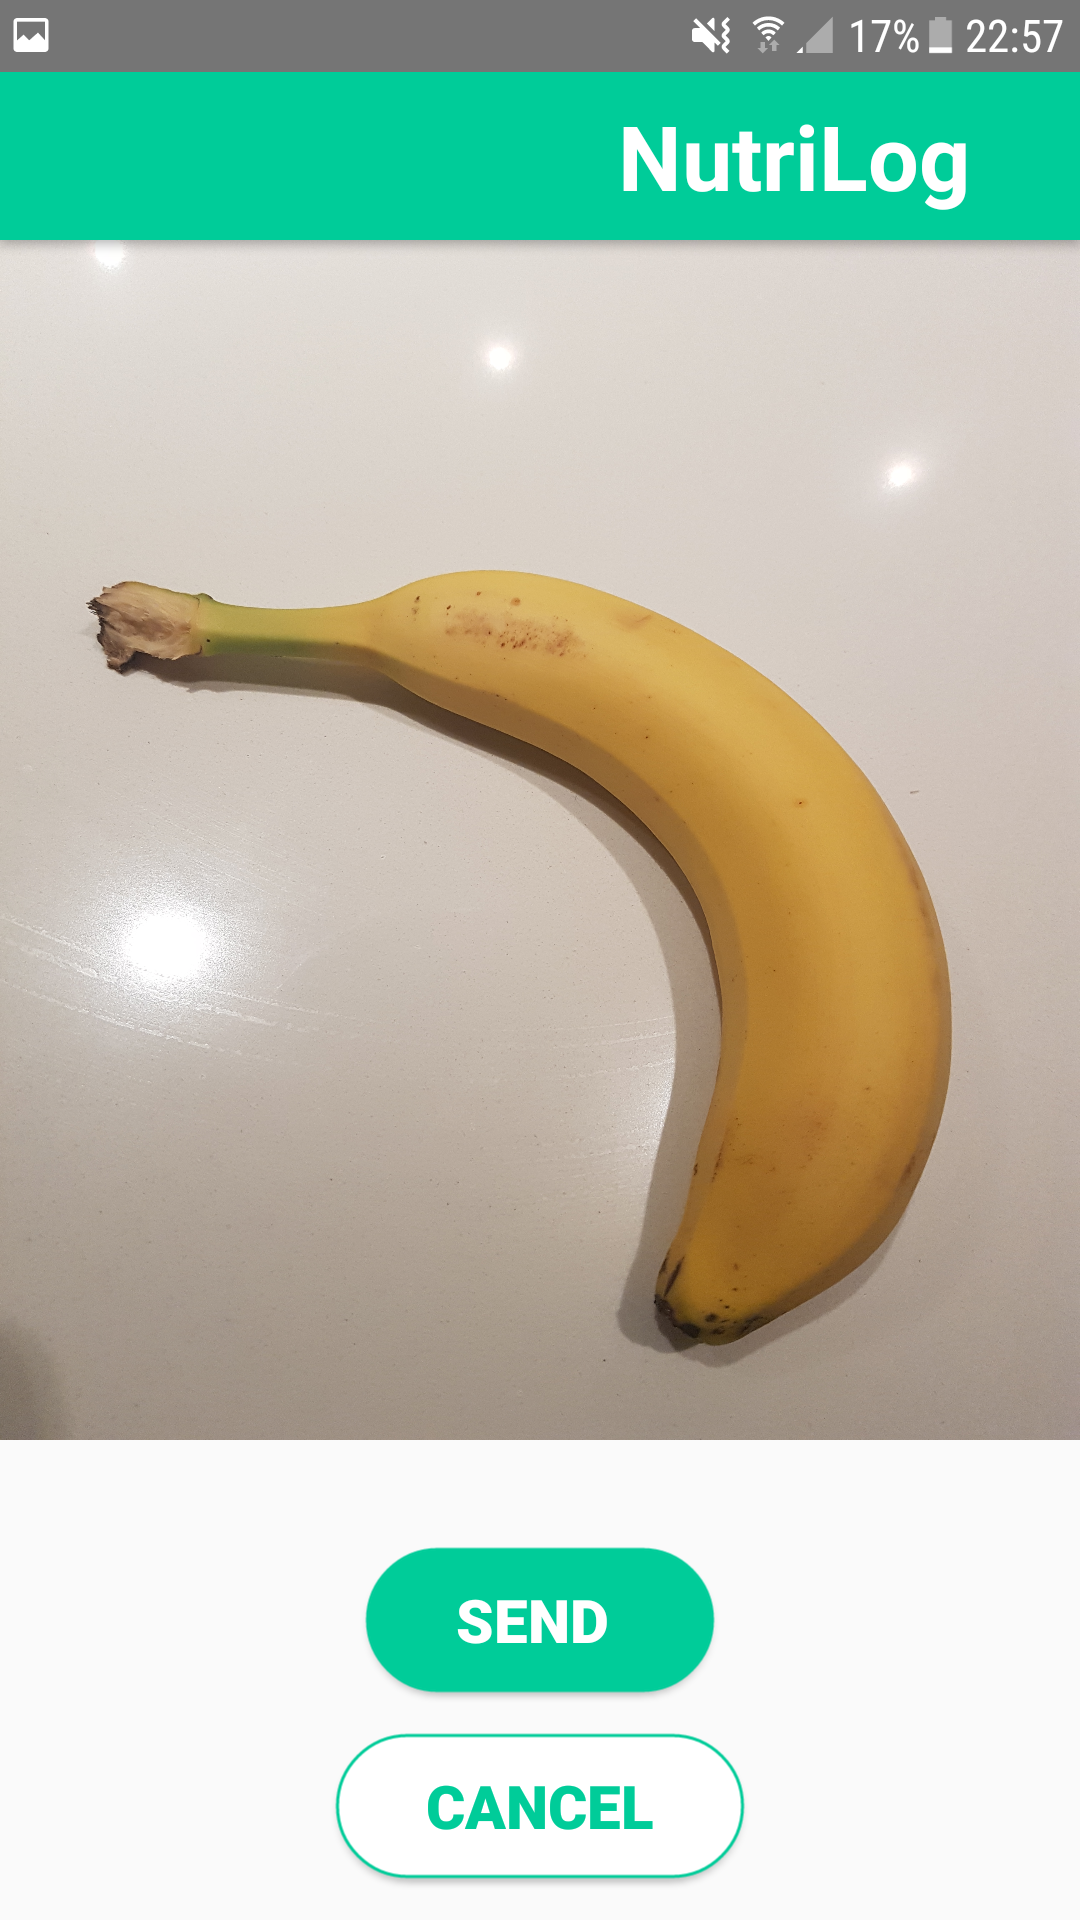
\includegraphics[width=.75\linewidth]{ui3} 
    \caption{Image Send Activity} 
    \label{fig:ui3}
    \vspace{4ex}
  \end{minipage}%% 
  \begin{minipage}[b]{0.5\linewidth}
    \centering
    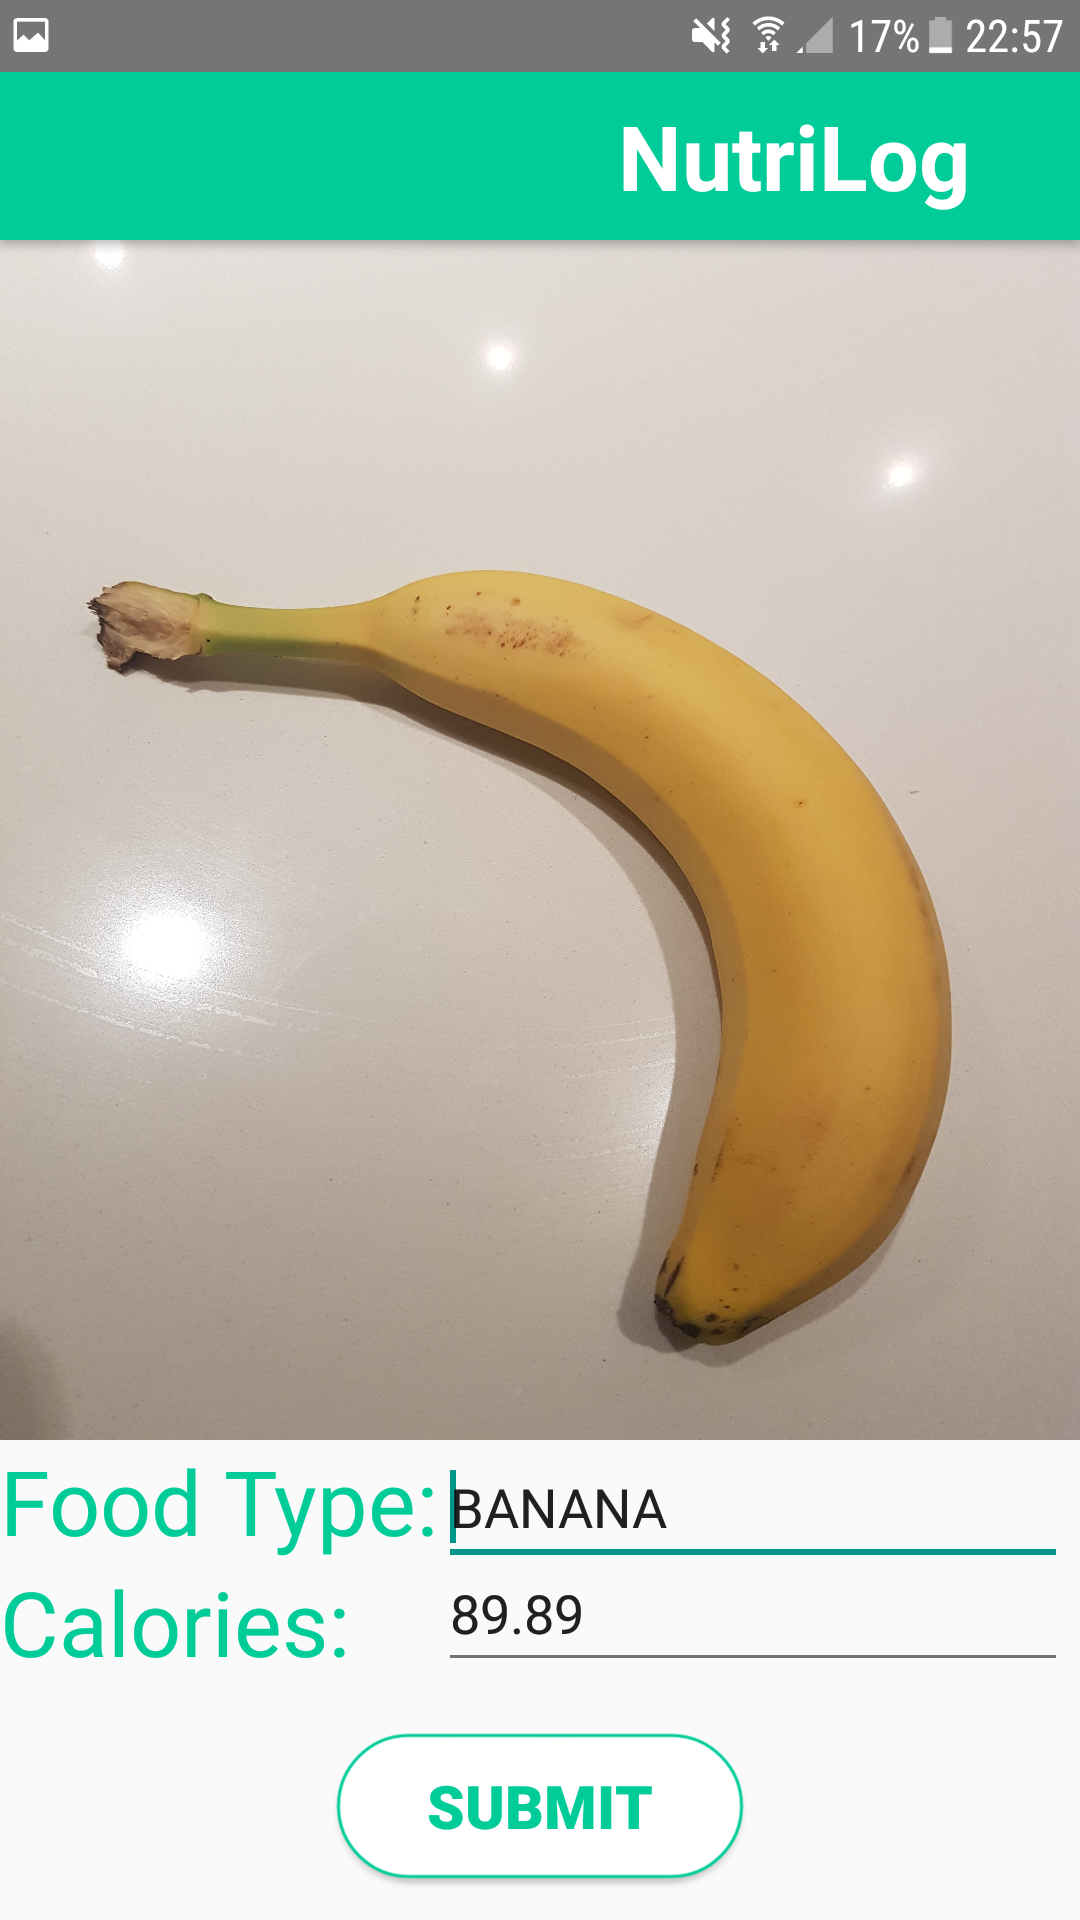
\includegraphics[width=.75\linewidth]{ui5} 
    \caption{Image Submit Activity} 
    \label{fig:ui5}
    \vspace{4ex}
  \end{minipage} 
\end{figure}

\begin{figure}
  \label{uiDesign2} 
  \begin{minipage}[b]{0.5\linewidth}
    \centering
    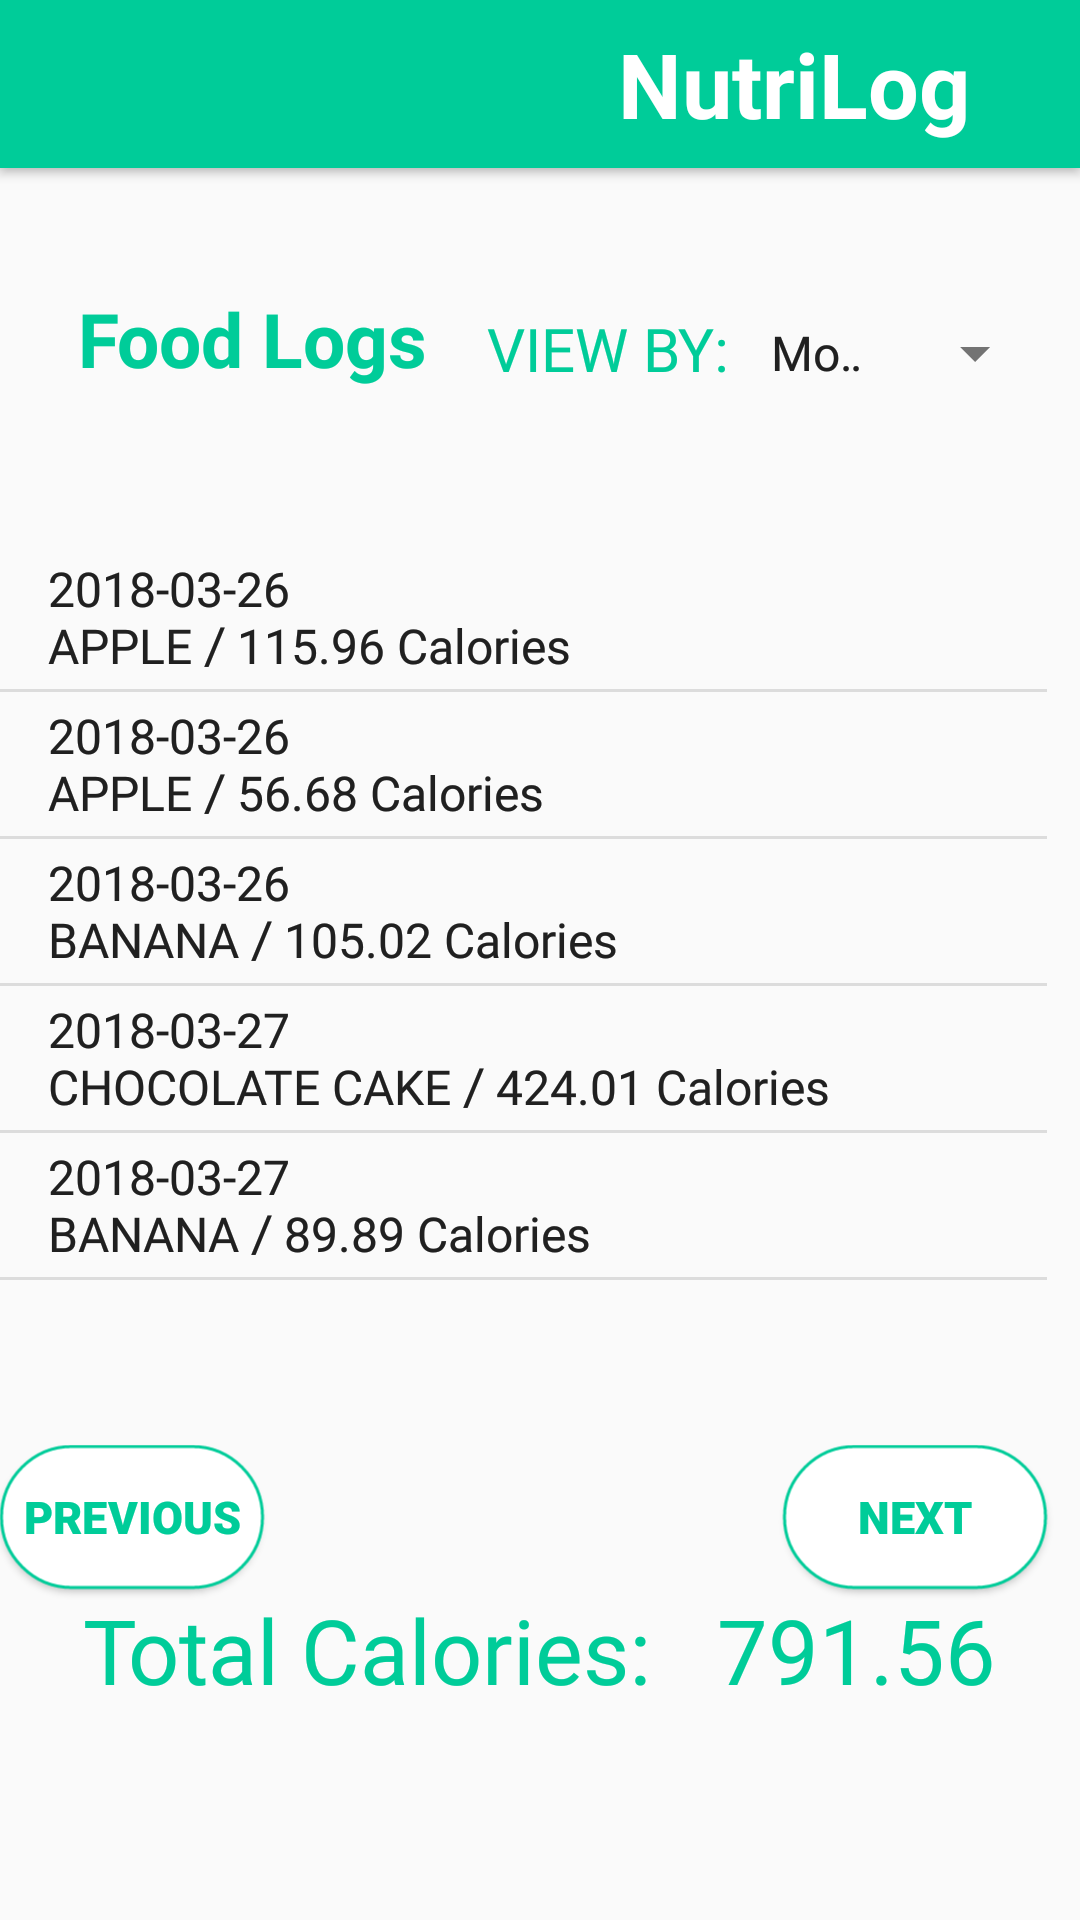
\includegraphics[width=.75\linewidth]{ui8} 
    \caption{FoodLog Month Activity} 
    \label{fig:ui8}
    \vspace{4ex}
  \end{minipage}
  \begin{minipage}[b]{0.5\linewidth}
    \centering
    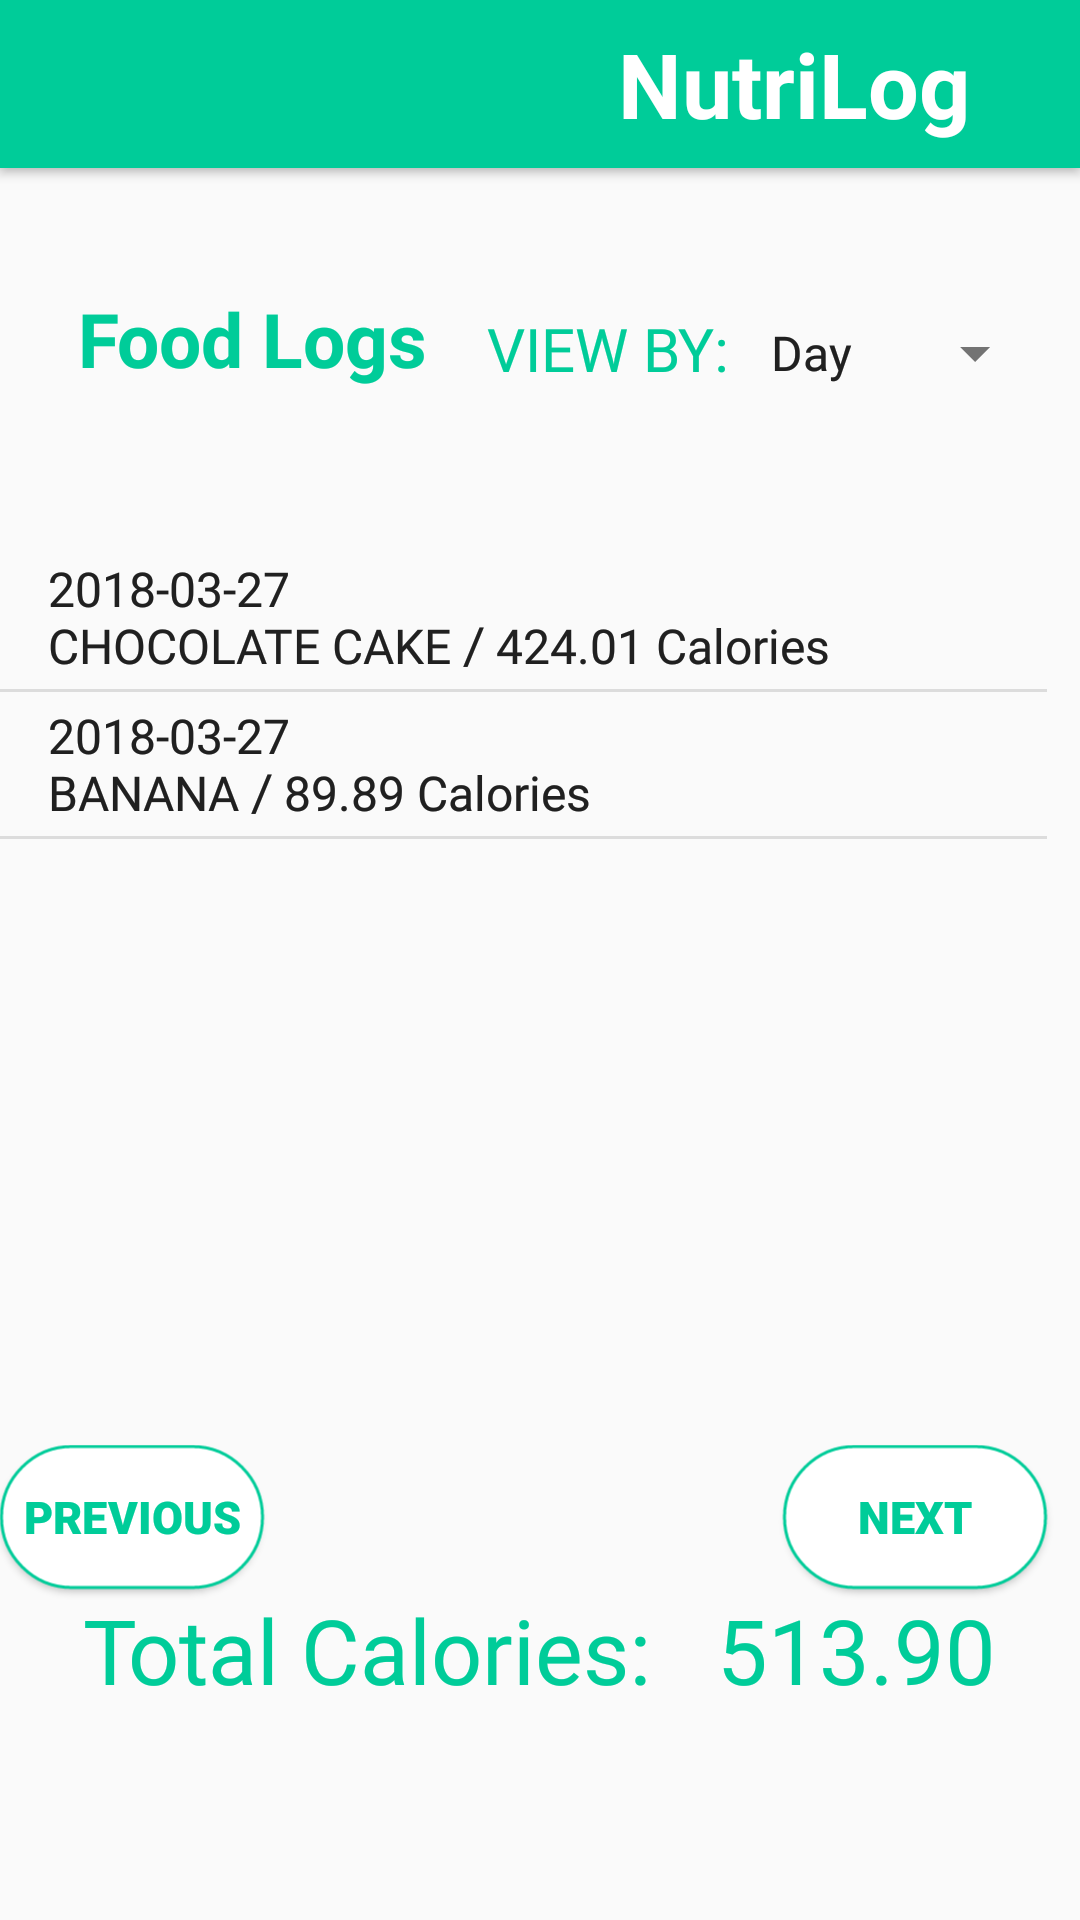
\includegraphics[width=.75\linewidth]{ui6} 
    \caption{FoodLog Day Activity} 
  \label{fig:ui6}
    \vspace{4ex}
  \end{minipage} 
  \begin{minipage}[b]{0.5\linewidth}
    \centering
    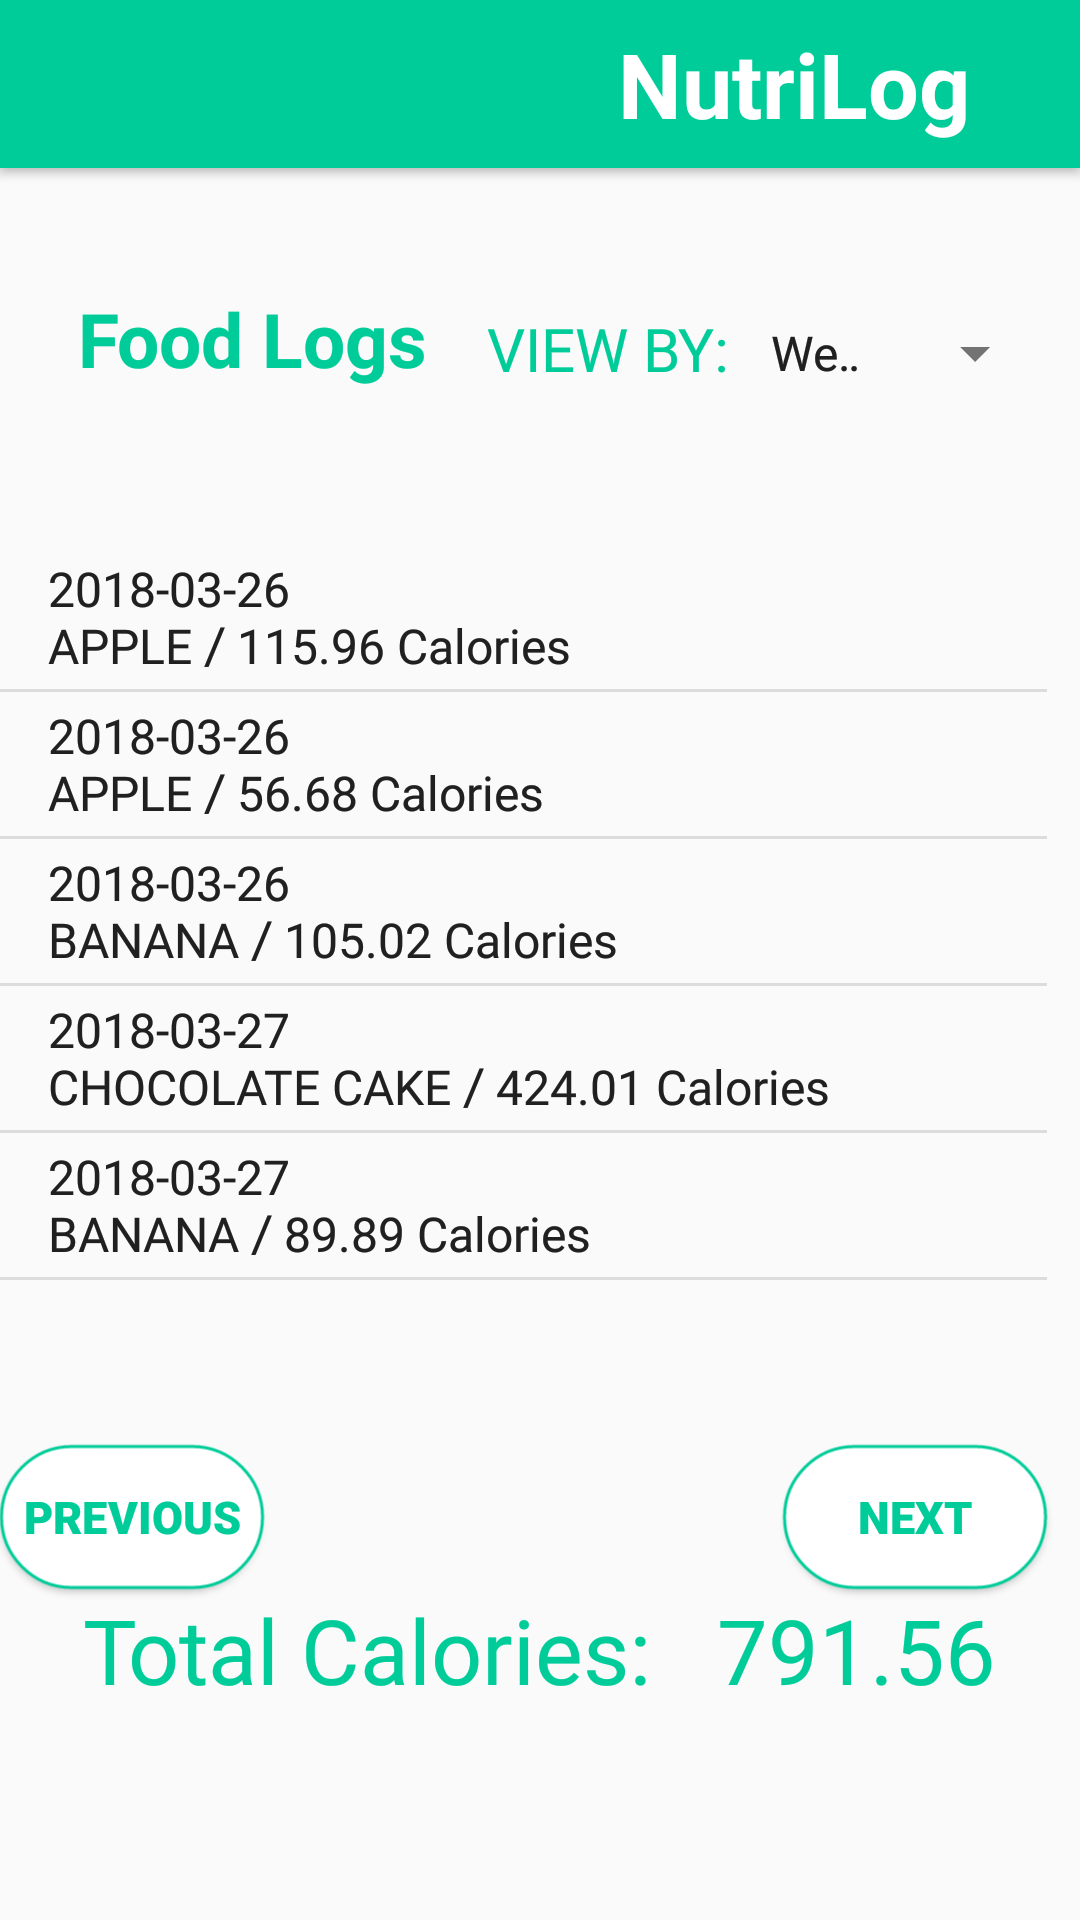
\includegraphics[width=.75\linewidth]{ui7} 
    \caption{FoodLog Week Activity} 
    \label{fig:ui7}
    \vspace{4ex}
  \end{minipage}%% 
  \begin{minipage}[b]{0.5\linewidth}
    \centering
    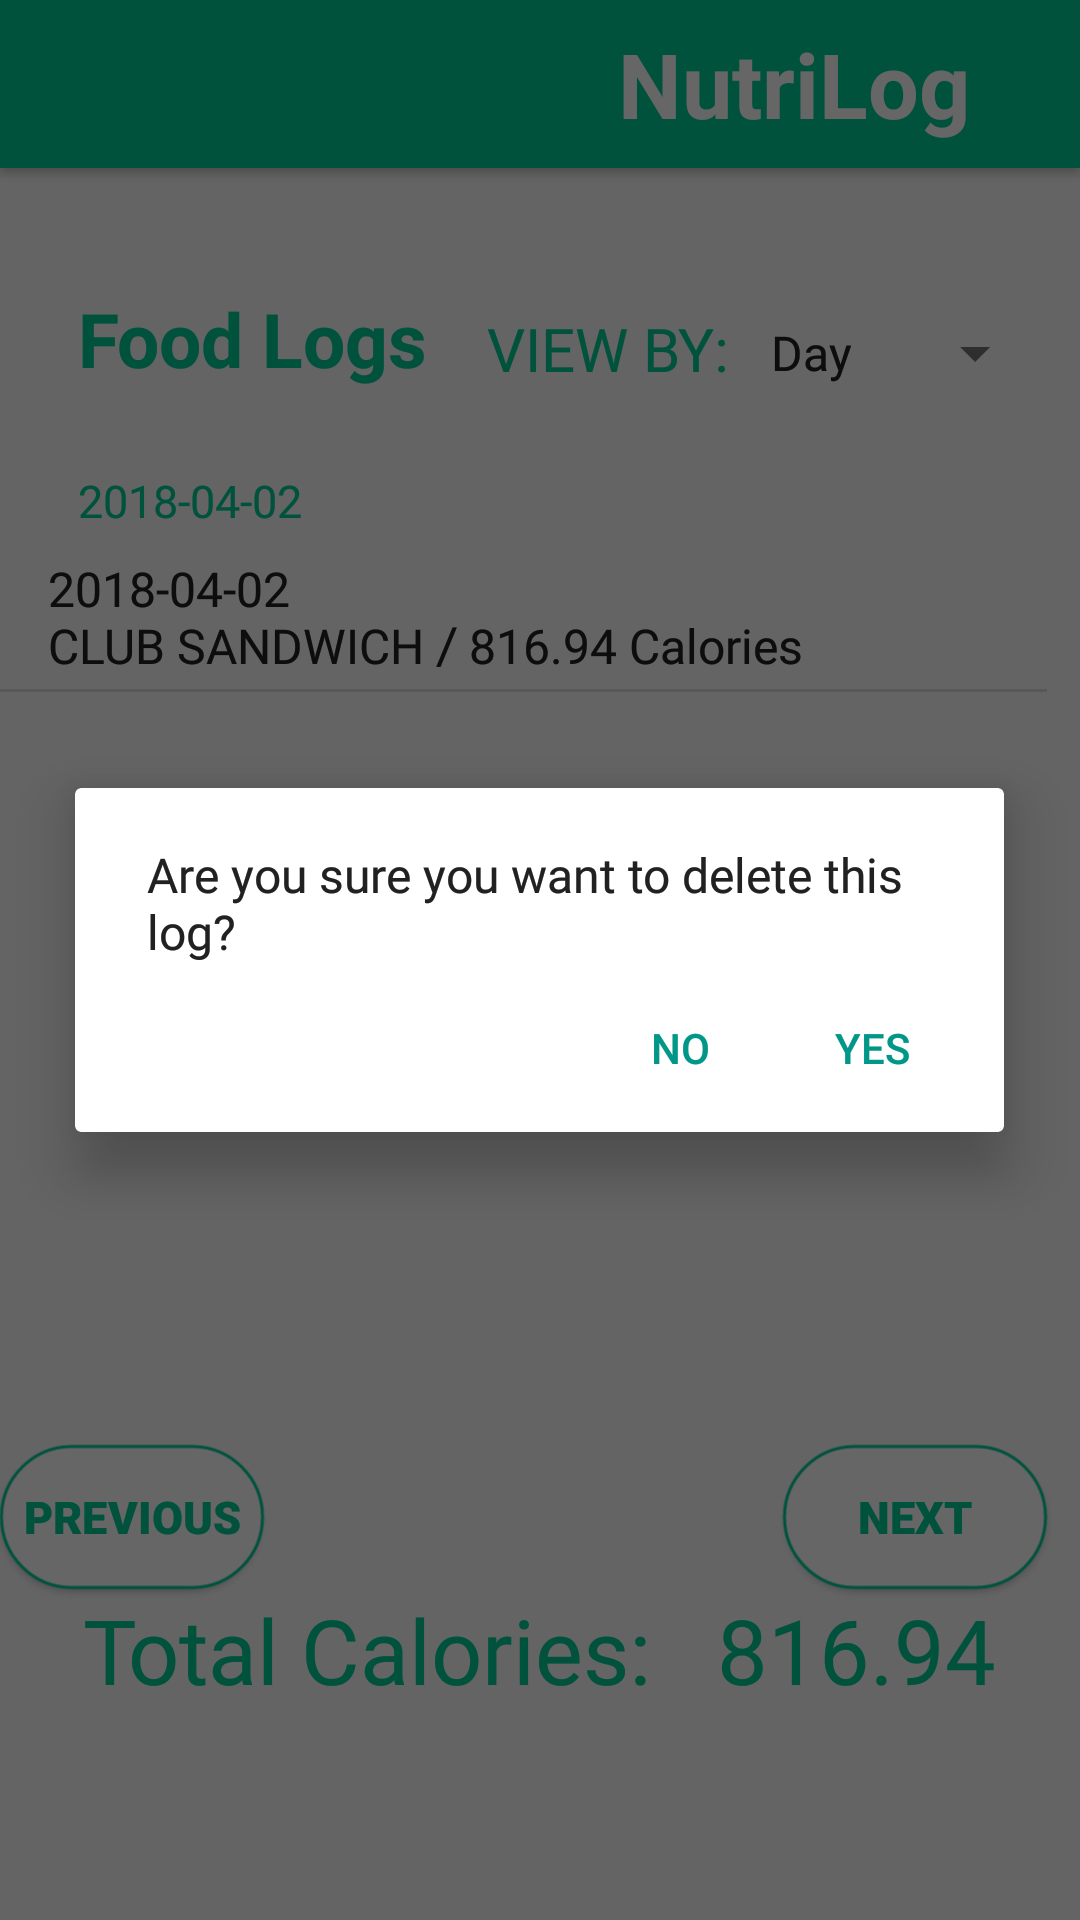
\includegraphics[width=.75\linewidth]{delete} 
    \caption{Food Log Deletion} 
  \label{fig:delete}
    \vspace{4ex} 
    \end{minipage}%% 
\end{figure}
\clearpage

\tocless\subsection{Technologies}

\tocless\subsubsection{GitHub}
GitHub was used as the version control backup system for this project.
Commit history can be seen in Figure \ref{fig:git}

\begin{figure}[h]
    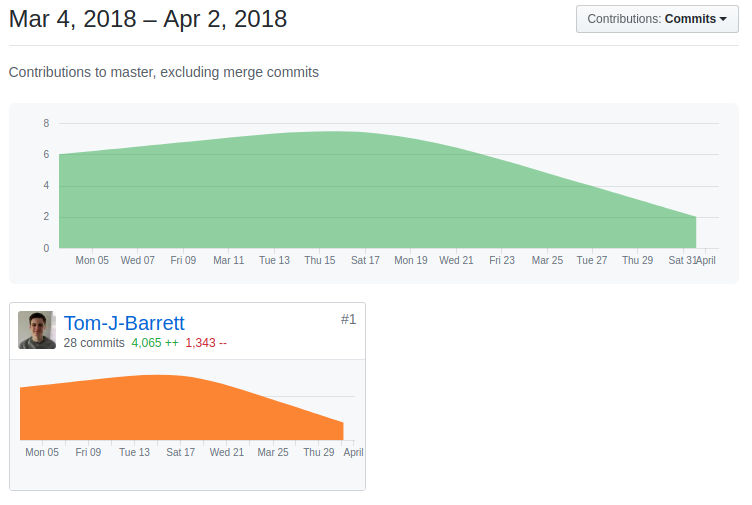
\includegraphics[scale=0.5]{git}
    \caption{GitHub Contributions to Master}
    \label{fig:git}
\end{figure}

\tocless\subsubsection{JSON}
JSON (JavaScript Object Notation) is a text format used to store data \parencite{json}.
It is both easy for machines to parse and for humans to read and write.
It is a data-interchange format as it is language independent.
JSON data structures are built on key pairs values and are normally parsed into arrays, lists or vectors.

\tocless\subsubsection{OkHttp}
OkHttp is a HTTP client created specifically for Java and Android applications \parencite{okhttp}.
It is a very efficient HTTP client with inbuilt defense against troublesome networks (recovers from common problems silently).
Some of the efficiency components are as follows:
\begin{itemize}
    \item{HTTP/2 support.}
    \item{Reduced request latency due to connection pooling.}
    \item{Caching of responses.}
\end{itemize}

\tocless\subsubsection{Nutritionix API}
The Nutritionix API is an API used to collect nutritional information \parencite{nutritionix}.
This project used this API to collect calorie information on a food item.
The free 'Hacker' account can support up to 10 active users.

\tocless\subsection{Software Quality Attributes}
Two main software quality attributes were focused on during the implementation of this prototype application. These were extensibility and maintainability.

Extensibility defines how easy it is to extend the functionality of the system.
There were certain places where the system developed is highly extensible.
A factory class was used to get the data access object that was used to store information in the application.
This factory class has a factory method that returns a DAO object which is an interface.
If the developer of the system needs to create an alternative way to store data in the application, they can create an object that implements the DAO interface and replace one line of code in the factory class.
A factory class was also used to create a Host object with the same rationale.

Maintainability defines how easy it is to maintain a system.
The system is maintainable for many reasons.
These reasons include low coupling, high cohesion and readability.






\section{Testing}
JUnit tests were used to test this prototype application.
JUnit is a unit testing framework.
Mockito is a framework for JUnit that was also utilised.
Mockito makes mocks of objects for testing.
This is very useful to test database instances as you can mock an SQLite Database object.

\tocless\subsection{Unit Tests}
Evidence of some unit tests written for this prototype application can be seen in Figures \ref{lst:test1}, \ref{lst:test2} and \ref{lst:test3}.
Figure \ref{fig:unitTests} also displays the automated tests that were run from Android Studio.

\begin{figure}[h]
    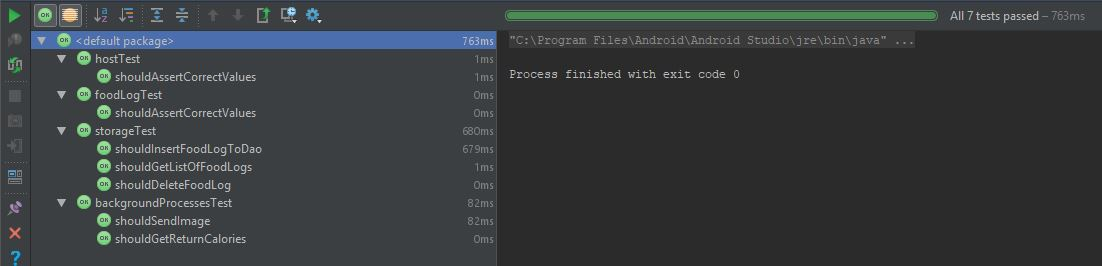
\includegraphics[scale=0.5]{UnitTests}
    \caption{Automated Unit Tests}
    \label{fig:unitTests}
\end{figure}

\begin{figure}[h]
\caption{Test to ensure FoodLog object stores information correctly}
\label{lst:test1}
\begin{lstlisting}[style=Java]
@Before
public void setUp() {
    foodLog = new FoodLogImpl(0, "banana", 59.03, new Date());
}

@Test
public void shouldAssertCorrectValues() {
    assert food.equals(foodLog.getFood());
    assert calories == foodLog.getCalories();
    assert timestamp.equals(foodLog.getTimestamp());
    assert id == foodLog.getId();
}
\end{lstlisting}
\end{figure}

\begin{figure}[h]
\caption{Test to ensure Host object stores information correctly}
\label{lst:test2}
\begin{lstlisting}[style=Java]
@Before
    public void setUp() {
        host = new Host.HostBuilder("52.214.205.157")
                .withDns("ec2-52-214-205-157.eu-west-1.compute.amazonaws.com")
                .withPort(5000)
                .withRoute("/classifyImage/")
                .build();
    }

@Test
public void shouldAssertCorrectValues() {
    assert this.ip.equals(host.getIpv4());
    assert this.dns.equals(host.getDns());
    assert this.port == host.getPort();
    assert this.route.equals(host.getRoute());
    assert this.urlString.equals(host.getUrl());
}
\end{lstlisting}
\end{figure}

\begin{figure}[h]
\caption{Test to ensure DAO object stores and removes data correctly}
\label{lst:test3}
\begin{lstlisting}[style=Java]
@Before
public void setup() {
    dao = mock(SqlLiteDAO.class);
    date = new Date();
    foodLog = new FoodLogImpl(0, "test", 0.0, date);
}

@Test
public void shouldGetListOfFoodLogs() {
    foodLogs = dao.getLogsByDay(date);
    foodLogs = dao.getLogsByWeek(date);
    foodLogs = dao.getLogsByMonth(date);
}

@Test
public void shouldInsertFoodLogToDao() {
    dao.addFoodLog(foodLog);
    setTestLog();
    assert foodLogs.contains(testLog);
}

@Test
public void shouldDeleteFoodLog() {
    List<FoodLog> foodLogs = new ArrayList<>();
    foodLogs.add(testLog);
    dao.deleteFoodLogs(foodLogs);
    setTestLog();
    assert testLog.equals(null);
}

private void setTestLog() {
    foodLogs = dao.getLogsByDay(date);
    foodLogs.forEach(f -> {
        if(f.getFood().equals("test")) {
            testLog = f;
        }
    });
}
\end{lstlisting}
\end{figure}

\clearpage

\section{Backend}
\tocless\subsection{Python Flask}

\tocless\subsection{Implementation}
Figures \ref{lst:backendCode} and \ref{lst:labelBackend} document the code used to implement the backend service.

\begin{figure}[h]
\caption{Backend service code}
\label{lst:backendCode}
\begin{lstlisting}[style=Python]
import base64
import label_image
import time

app = Flask(_name_)

#add a route for the flask app and what HTTP methods are allowed
@app.route('/classifyImage/', methods=['POST'])
def classify():
    #decode image and save it
    imgdata = base64.b64decode(request.form.get('image'))
    filename = 'images/' + str(time.strftime("%Y%m%d-%H%M%S")) + '.jpg'
    with open(filename, 'wb') as f:
        f.write(imgdata)

    #classify the image
    results = label_image.runModel(filename)
    predictions = results[0]

    #retrun a String of the results
    result_String = ""
    for i in predictions :
        result_String += str(i) + ","
    return result_String

#runs the app on port 5000
if _name_ == '_main_':
    app.run(host='0.0.0.0', threaded=True)
\end{lstlisting}
\end{figure}

\begin{figure}[h]
\caption{Method called from 'label\_image.py' - adapted from \parencite{retrainInception}}
\label{lst:labelBackend}
\begin{lstlisting}[style=Python]
def runModel(file_name):
  #hardcoded values of image size and model path
  model_file = \
    "models/output_graph13.pb"
  label_file = "labels/output_labels13.txt"
  input_height = 299
  input_width = 299
  input_mean = 128
  input_std = 128
  input_layer = "Mul"
  output_layer = "final_result"

  #load the graph using load_graph() provided be Google
  graph = load_graph(model_file)
  #read in tensor
  t = read_tensor_from_image_file(file_name,
                                  input_height=input_height,
                                  input_width=input_width,
                                  input_mean=input_mean,
                                  input_std=input_std)

  input_name = "import/" + input_layer
  output_name = "import/" + output_layer
  input_operation = graph.get_operation_by_name(input_name)
  output_operation = graph.get_operation_by_name(output_name)

  #run the tensor through the graph
  with tf.Session(graph=graph) as sess:
    results = sess.run(output_operation.outputs[0],
                      {input_operation.outputs[0]: t})
  results = np.squeeze(results)

  #get the top 5 results
  top_k = results.argsort()[-5:][::-1]
  labels = load_labels(label_file)

  setIndex = False

  #return results
  top5_results = [None] * 5
  index = 0
  for i in top_k:
    top5_results[index] = labels[i]
    index += 1

  final_results = [top5_results, results]
  return final_results
\end{lstlisting}
\end{figure}

\tocless\subsection{Deployment}
In order to deploy the Flask application to an AWS EC2 instance the following steps had to be followed:

\begin{itemize}
    \item{Upload the output\_graph.pb file (TensorFlow model), the output\_labels.txt file and the source code to the server using SFTP.}
    \item{SSH into the server.}
    \item{Create a folder called 'images' in the home directory to store uploads images.}
    \item{Place model and label files into folders called 'models' and 'labels' respectively.}
    \item{Ensure TensorFlow, Python and Flask are installed on the server.}
    \item{Ensure no processes are running on port 5000 using the command 'lsof -i :5000'.}
    \item{Use the command 'screen'.}
    \item{Run the server.py code using the command 'python server.py'.}
    \item{Use the commands CTRL+A and CRTL+D to exit screen.}
\end{itemize}

\tocless\subsubsection{AWS Architecture}
The application interfaces with an Amazon Web Services (AWS) server called an EC2 instance.
To keep the application secure AWS was used to provide a secure architecture.
A Virtual Private Cloud (VPC) was created to host the instances.
In a production environment a load balancer could be used to evenly distribute traffic across a fleet of backend instances but for the purposes of this prototype application, a single instance as in Figure \ref{fig:aws} could be used.
In Figure \ref{fig:aws} the instance is located inside a subnet which is in turn located in a VPC.
The purpose of a VPC is to have a virtual network dedicated to a users individual account. 
\begin{figure}[h]
    \centering
    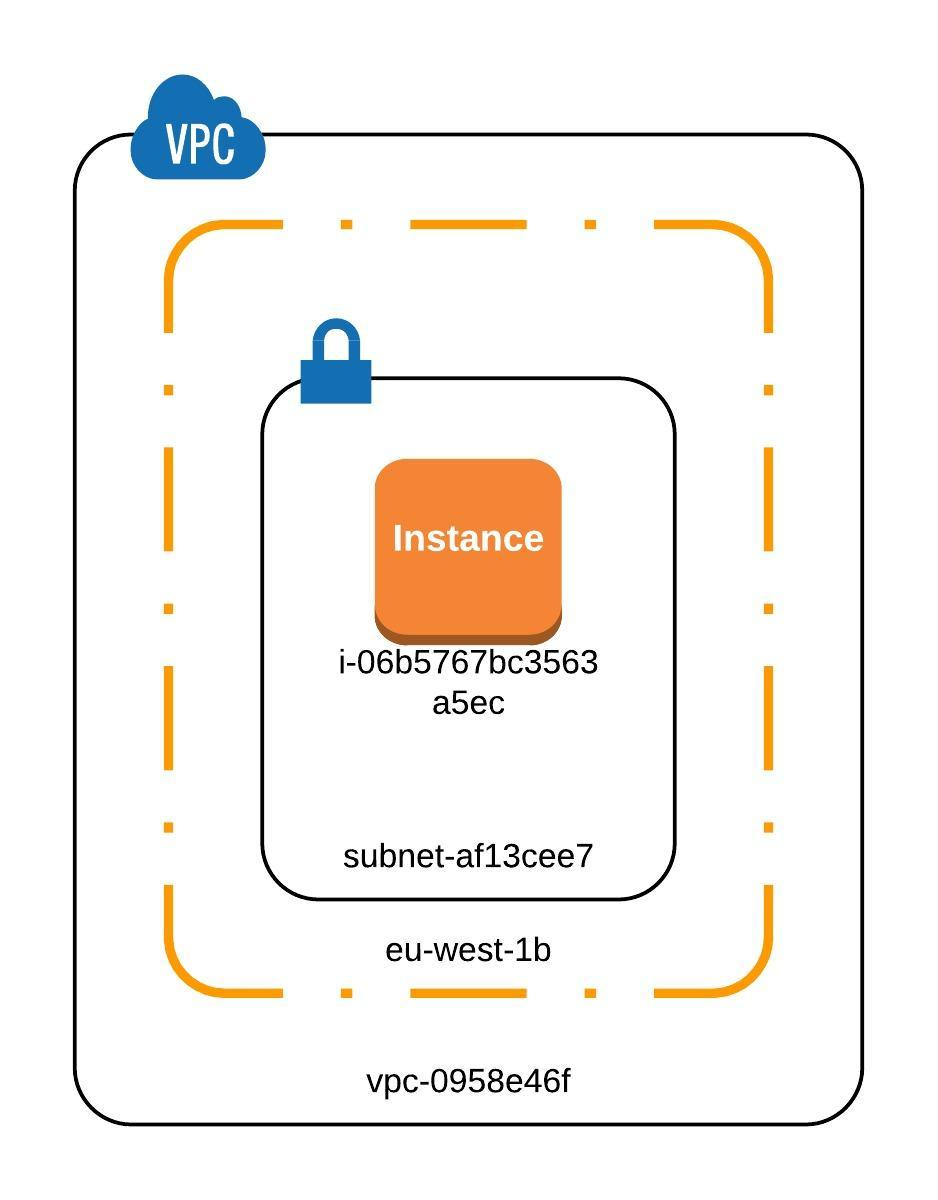
\includegraphics{aws}
    \caption{AWS Network Diagram}
    \label{fig:aws}
\end{figure}

Security groups were utilised to restrict the type of traffic that would be allowed to reach the instance, so that the instance would only receive HTTP requests at port 5000 and receive SSH connections at port 22 as per Figure \ref{fig:awsSecGroup}.
\begin{figure}[h]
    \centering
    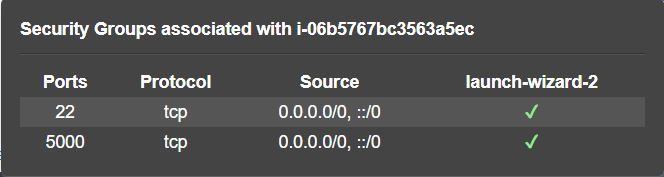
\includegraphics{secGroups}
    \caption{AWS Security Group}
    \label{fig:awsSecGroup}
\end{figure}

% \begin{itemize}
%     \item{Upload the output_graph.pb file (Tensorflow model), the output_labels.txt file and the source code to the server using SFTP}
%     \item{SSH into the server}
%     \item{Create a folder called 'images' in the home directory to store uploads images}
%     \item{Place model and label files into folders called 'models' and 'labels' respectively}
%     \item{Ensure Tensorflow, NOHUP (Ignores the hangup signal in Linux) Python and Flask are installed on the server}
%     \item{Ensure no processes are running on port 5000 using the command 'lsof -i :5000'}
%     \item{Run the server.py code using the command 'nohup python server.py &'}
% \end{itemize}

\section{Resources Utilised}
\input{tex/prototype/resources}
